% Capitolul 9: Modele ARCH și GARCH
% Statistica piețelor financiare -- Program de licență, Academia de Studii Economice din București
% GENERAT de latex/build_chapter9.py -- modificați generatorul, nu acest fișier.

\newcommand{\coursename}{Statistica piețelor financiare}
\def\sfmlang{ro}
% Preambul comun SFM -- Statistica piețelor financiare / Statistics of Financial Markets (Beamer, 16:9)
% Același design ca MFM. Înainte de % Preambul comun SFM -- Statistica piețelor financiare / Statistics of Financial Markets (Beamer, 16:9)
% Același design ca MFM. Înainte de % Preambul comun SFM -- Statistica piețelor financiare / Statistics of Financial Markets (Beamer, 16:9)
% Același design ca MFM. Înainte de \input{../../latex/preamble} se definește
%   \newcommand{\coursename}{Statistics of Financial Markets}      (EN)
%   \newcommand{\coursename}{Statistica piețelor financiare}       (RO)  și  \def\sfmlang{ro}
% Fișierele .tex se află în EN/Courses, EN/Seminars, RO/Cursuri, RO/Seminarii (două niveluri sub rădăcină).
% Deck-urile sînt generate de latex/build_chapterN.py / build_seminarN.py (vezi latex/sfm_build.py).

\documentclass[9pt, aspectratio=169, t]{beamer}
\providecommand{\coursename}{Statistics of Financial Markets}

% Ensure content fits on slides
\setbeamersize{text margin left=8mm, text margin right=8mm}

%=============================================================================
% THEME AND STYLE CONFIGURATION
%=============================================================================
\usetheme{default}
% Using default theme for clean header/footer control

% Color Palette (matching Redispatch PDF)
\definecolor{MainBlue}{RGB}{26, 58, 110}
\definecolor{AccentBlue}{RGB}{26, 58, 110}
\definecolor{IDAred}{RGB}{205, 0, 0}
\definecolor{DarkGray}{RGB}{51, 51, 51}
\definecolor{MediumGray}{RGB}{128, 128, 128}
\definecolor{LightGray}{RGB}{248, 248, 248}
\definecolor{VeryLightGray}{RGB}{235, 235, 235}
\definecolor{KeynoteGray}{RGB}{218, 218, 218}
\definecolor{SectionGray}{RGB}{120, 120, 120}
\definecolor{FooterGray}{RGB}{100, 100, 100}
\definecolor{Crimson}{RGB}{220, 53, 69}
\definecolor{Forest}{RGB}{46, 125, 50}
\definecolor{Amber}{RGB}{181, 133, 63}
\definecolor{Orange}{RGB}{230, 126, 34}
\definecolor{Purple}{RGB}{142, 68, 173}

% Gradient background (exact Keynote 315° gradient: white to RGB 218,218,218)
\setbeamertemplate{background}{%
    \begin{tikzpicture}[remember picture, overlay]
        \shade[shading=axis, shading angle=315,
        top color=white, bottom color=KeynoteGray]
        (current page.south west) rectangle (current page.north east);
    \end{tikzpicture}%
}
% Fallback solid color for compatibility
\setbeamercolor{background canvas}{bg=}

\setbeamercolor{palette primary}{bg=MainBlue, fg=white}
\setbeamercolor{palette secondary}{bg=MainBlue!85, fg=white}
\setbeamercolor{palette tertiary}{bg=MainBlue!70, fg=white}
\setbeamercolor{structure}{fg=MainBlue}
\setbeamercolor{title}{fg=IDAred}
\setbeamercolor{frametitle}{fg=IDAred, bg=}
\setbeamercolor{block title}{bg=MainBlue, fg=white}
\setbeamercolor{block body}{bg=VeryLightGray, fg=DarkGray}
\setbeamercolor{block title alerted}{bg=Crimson, fg=white}
\setbeamercolor{block body alerted}{bg=Crimson!8, fg=DarkGray}
\setbeamercolor{block title example}{bg=Forest, fg=white}
\setbeamercolor{block body example}{bg=Forest!8, fg=DarkGray}
\setbeamercolor{item}{fg=MainBlue}

% Footer colors (override Madrid theme blue)
\setbeamercolor{author in head/foot}{fg=FooterGray, bg=}
\setbeamercolor{title in head/foot}{fg=FooterGray, bg=}
\setbeamercolor{date in head/foot}{fg=FooterGray, bg=}
\setbeamercolor{section in head/foot}{fg=FooterGray, bg=}
\setbeamercolor{subsection in head/foot}{fg=FooterGray, bg=}

% Bullet styles (apply everywhere including blocks)
\setbeamertemplate{itemize item}{\color{MainBlue}$\boxdot$}
\setbeamertemplate{itemize subitem}{\color{MainBlue}$\blacktriangleright$}
\setbeamertemplate{itemize subsubitem}{\color{MainBlue}\tiny$\bullet$}
\setbeamertemplate{itemize/enumerate body begin}{\normalsize}
\setbeamertemplate{itemize/enumerate subbody begin}{\normalsize}

% Item spacing - compact style
\setlength{\leftmargini}{10pt}       % Level 1: minimal indent
\setlength{\leftmarginii}{10pt}      % Level 2: minimal additional indent
% Compact list spacing (zero extra space before/after lists in blocks)
\makeatletter
\def\@listi{\leftmargin\leftmargini \topsep 0pt \parsep 0pt \itemsep 0pt}
\def\@listii{\leftmargin\leftmarginii \topsep 0pt \parsep 0pt \itemsep 0pt}
\makeatother

\setbeamertemplate{navigation symbols}{}

%=============================================================================
% CUSTOM HEADLINE
%=============================================================================
\setbeamertemplate{headline}{%
    \vskip10pt%
    \hbox to \paperwidth{%
        \hskip0.5cm%
        {\small\color{FooterGray}\renewcommand{\hyperlink}[2]{##2}\insertsectionhead}%
        \hfill%
        \textcolor{FooterGray}{\small\insertframenumber}%
        \hskip0.5cm%
    }%
    \vskip4pt%
    {\color{FooterGray}\hrule height 0.4pt}%
}

%=============================================================================
% CUSTOM FOOTER
%=============================================================================
\usepackage{fontawesome5}

\setbeamertemplate{footline}{%
    {\color{FooterGray}\hrule height 0.4pt}%
    \vskip4pt%
    \hbox to \paperwidth{%
        \hskip0.5cm%
        \textcolor{FooterGray}{\small\coursename}%
        \hfill%
        \raisebox{-0.1em}{%
            \begin{tikzpicture}[x=0.08em, y=0.08em, line width=0.4pt]
                \draw[FooterGray] (0,3) -- (1,4) -- (2,3.5) -- (3,5) -- (4,4) -- (5,6) -- (6,5.5) -- (7,4) -- (8,5) -- (9,7) -- (10,6) -- (11,5) -- (12,6.5) -- (13,8) -- (14,7) -- (15,6) -- (16,7.5) -- (17,9) -- (18,8) -- (19,7) -- (20,8.5) -- (21,10) -- (22,9) -- (23,8) -- (24,9.5);
            \end{tikzpicture}%
        }%
        \hskip0.5cm%
    }%
    \vskip6pt%
}

%=============================================================================
% PACKAGES
%=============================================================================
\usepackage[utf8]{inputenc}
\DeclareUnicodeCharacter{03B1}{\ensuremath{\alpha}}
\usepackage[T1]{fontenc}
\usepackage{amsmath, amssymb, amsthm}
\usepackage{mathtools}
\usepackage{bm}
\usepackage{tikz}
\usetikzlibrary{arrows.meta, positioning, shapes, calc, decorations.pathreplacing, shadings}
\usepackage{booktabs}
\usepackage{multirow}
\usepackage{array}
\usepackage{graphicx}
\usepackage{hyperref}
\usepackage{colortbl}
\usepackage{listings}
\lstset{language=Python, basicstyle=\ttfamily\scriptsize, keywordstyle=\color{MainBlue}\bfseries,
  commentstyle=\color{Forest}, stringstyle=\color{Crimson}, breaklines=true,
  frame=none, backgroundcolor=\color{VeryLightGray}, xleftmargin=2mm}
\hypersetup{colorlinks=true, linkcolor=MainBlue, urlcolor=MainBlue}
\graphicspath{{../../logos/}{../../charts/}{../../photos/}}
\usepackage{xcolor}
\hfuzz=2pt  % Suppress tiny overfull warnings (<2pt)
\vfuzz=2pt  % Suppress tiny vertical overfull warnings (<2pt)

%=============================================================================
% QUANTLET COMMANDS
%   \quantlet{<displayed name>}{<url>}       (generic, compatible with the older SFM decks)
%   \sfmquantlet{Ch_05}{SFM_ch5_garch}       -> https://github.com/danpele/SFM/tree/main/Quantlets/Ch_05/SFM_ch5_garch
%   \qlurl{<folder>} is defined per chapter by the generator (Quantlets/Ch_NN/<folder>)
%=============================================================================
\newcommand{\sfmrepo}{https://github.com/danpele/SFM}
\newcommand{\sfmqlbase}{https://github.com/danpele/SFM/tree/main/Quantlets}
\newcommand{\quantlet}[2]{%
    \hfill\href{#2}{%
        \raisebox{-0.15em}{
\includegraphics[height=0.7em]{ql_logo.png}}%
        \textcolor{MainBlue}{\tiny\ #1}%
    }%
}
\newcommand{\sfmquantlet}[2]{\quantlet{\detokenize{#2}}{\sfmqlbase/#1/#2}}

%=============================================================================
% NOTEBOOKS (Google Colab)
%   \colaburl{notebooks/EN/chapter5_seminar_notebook.ipynb} -> the Colab link of a file in the SFM repo
%   \nb: the chapter notebook (each seminar deck redefines it with \renewcommand)
%=============================================================================
\newcommand{\colaburl}[1]{https://colab.research.google.com/github/danpele/SFM/blob/main/#1}
\newcommand{\nb}{https://colab.research.google.com/github/danpele/SFM/tree/main/notebooks/EN}
\newcommand{\nbname}{notebooks/EN}

%=============================================================================
% SLIDE HELPERS (used by the generators; the same as in MFM)
%=============================================================================
% local font size for list bodies (the preamble forces \normalsize)
\newcommand{\itemsize}[1]{\setbeamertemplate{itemize/enumerate body begin}{#1}\setbeamertemplate{itemize/enumerate subbody begin}{#1}}
\newcommand{\intitle}[1]{{\hypersetup{urlcolor=white}#1}}   % white links inside coloured title bars
\newcommand{\imgcap}[1]{{\scriptsize #1}\\[0.5mm]}          % caption under a photo
\newcommand{\imgcredit}[2]{{\tiny\color{FooterGray}\href{#1}{#2}}}   % image credit: source URL, author/licence
\newcommand{\aiprompt}[1]{{\ttfamily\color{MainBlue}#1}}     % a prompt to an AI assistant

%=============================================================================
% SEMINARS: student version by default; the instructor wrapper *_solutions.tex sets \solutionstrue
%=============================================================================
\makeatletter\@ifundefined{ifsolutions}{\expandafter\newif\csname ifsolutions\endcsname}{}\makeatother
\newcommand{\solonly}[1]{\ifsolutions #1\fi}
\newcommand{\propsub}{\ifsolutions\else\framesubtitle{\ifdefined\sfmlang Rezolvarea se discută la seminar\else Solution discussed in class\fi}\fi}

%=============================================================================
% APPENDIX AND CHAPTER LINKS (latex/appendix_links.py writes the calls; it also re-declares these
% macros before \begin{document}, so the decks compile with or without this preamble block)
%=============================================================================
\providecommand{\sfmapplink}[3]{\hypertarget{#2}{}\hyperlink{#1}{\beamergotobutton{#3}}}
\providecommand{\sfmappback}[2]{\begin{tikzpicture}[remember picture,overlay]\node[anchor=south east] at ([xshift=-3mm,yshift=7mm]current page.south east){\hyperlink{#1}{\beamerreturnbutton{#2}}};\end{tikzpicture}}
\providecommand{\sfmchlink}[2]{\href{#1}{#2}}
\providecommand{\sfmchlinkt}[2]{\href{#1}{\usebeamercolor[fg]{frametitle}#2}}

%=============================================================================
% QUANTINAR COMMAND: link către un curs Quantinar (subiecte avansate)
%=============================================================================
\newcommand{\quantinar}[2]{%
    \href{#2}{%
        \raisebox{-0.15em}{
\includegraphics[height=0.8em]{qr_logo.png}}%
        \textcolor{MainBlue}{\scriptsize\ #1}%
    }%
}

%=============================================================================
% CUSTOM TITLE PAGE
%=============================================================================
\defbeamertemplate*{title page}{hybrid}[1][]
{
    \vspace{0.2cm}
    % Logos row - top header (with clickable links)
    \begin{center}
        \href{https://www.ase.ro}{
\includegraphics[height=1.0cm]{ase_logo.png}}\hspace{0.3cm}%
        \href{https://theida.net}{
\includegraphics[height=1.0cm]{ida_logo.png}}\hspace{0.3cm}%
        \href{https://blockchain-research-center.com}{
\includegraphics[height=1.0cm]{brc_logo.png}}\hspace{0.3cm}%
        \href{https://www.ai4efin.ase.ro}{
\includegraphics[height=1.0cm]{ai4efin_logo.png}}\hspace{0.3cm}%
        \href{https://ipe.ro/new}{
\includegraphics[height=1.0cm]{acad_logo.png}}\hspace{0.3cm}%
        \href{https://www.digital-finance-msca.com}{
\includegraphics[height=1.0cm]{msca_logo.png}}%
    \end{center}

    \vspace{0.6cm}

    % Main title with Q logos on sides (with clickable links)
    \begin{center}
        \begin{minipage}{0.1\textwidth}
            \centering
            \href{https://quantlet.com}{
\includegraphics[height=1.1cm]{ql_logo.png}}
        \end{minipage}%
        \begin{minipage}{0.78\textwidth}
            \centering
            {\LARGE\bfseries\usebeamercolor[fg]{title}\inserttitle}

            \vspace{0.3cm}

            {\usebeamerfont{subtitle}\usebeamercolor[fg]{title}\insertsubtitle}
        \end{minipage}%
        \begin{minipage}{0.1\textwidth}
            \centering
            \href{https://quantinar.com}{
\includegraphics[height=1.1cm]{qr_logo.png}}
        \end{minipage}
    \end{center}

    \vspace{0.6cm}

    % Authors (left aligned)
    \hspace{0.5cm}{\usebeamerfont{author}\insertauthor}

    \vspace{0.3cm}

    % Institute/Affiliations (left aligned)
    \hspace{0.5cm}\begin{minipage}[t]{0.9\textwidth}
        \raggedright\small\insertinstitute
    \end{minipage}
}

%=============================================================================
% THEOREM ENVIRONMENTS
%=============================================================================
\theoremstyle{definition}
\setbeamertemplate{theorems}[numbered]
\ifdefined\sfmlang
\newtheorem{defn}{Definiție}
\newtheorem{thm}{Teoremă}
\newtheorem{prop}{Propoziție}
\newtheorem{rmk}{Observație}
\else
\newtheorem{defn}{Definition}
\newtheorem{thm}{Theorem}
\newtheorem{prop}{Proposition}
\newtheorem{rmk}{Remark}
\fi

%=============================================================================
% CENTRED MINIPAGE (no extra vertical space)
%=============================================================================
\newenvironment{cminipage}[1]{%
    \par\noindent\hfill\begin{minipage}{#1}\ignorespaces
}{%
    \end{minipage}\hfill\null\par
}

%=============================================================================
% CUSTOM COMMANDS
%=============================================================================
\newcommand{\E}{\mathbb{E}}
\newcommand{\Var}{\text{Var}}
\newcommand{\Cov}{\text{Cov}}
\newcommand{\Corr}{\text{Corr}}
\newcommand{\R}{\mathbb{R}}
\newcommand{\N}{\mathbb{N}}
\newcommand{\Z}{\mathbb{Z}}
\newcommand{\B}{\mathbf{B}}
\newcommand{\imark}{\textcolor{MainBlue}{\textbullet}}
\newcommand{\RMSE}{\text{RMSE}}
\newcommand{\MAE}{\text{MAE}}
\newcommand{\MAPE}{\text{MAPE}}

 se definește
%   \newcommand{\coursename}{Statistics of Financial Markets}      (EN)
%   \newcommand{\coursename}{Statistica piețelor financiare}       (RO)  și  \def\sfmlang{ro}
% Fișierele .tex se află în EN/Courses, EN/Seminars, RO/Cursuri, RO/Seminarii (două niveluri sub rădăcină).
% Deck-urile sînt generate de latex/build_chapterN.py / build_seminarN.py (vezi latex/sfm_build.py).

\documentclass[9pt, aspectratio=169, t]{beamer}
\providecommand{\coursename}{Statistics of Financial Markets}

% Ensure content fits on slides
\setbeamersize{text margin left=8mm, text margin right=8mm}

%=============================================================================
% THEME AND STYLE CONFIGURATION
%=============================================================================
\usetheme{default}
% Using default theme for clean header/footer control

% Color Palette (matching Redispatch PDF)
\definecolor{MainBlue}{RGB}{26, 58, 110}
\definecolor{AccentBlue}{RGB}{26, 58, 110}
\definecolor{IDAred}{RGB}{205, 0, 0}
\definecolor{DarkGray}{RGB}{51, 51, 51}
\definecolor{MediumGray}{RGB}{128, 128, 128}
\definecolor{LightGray}{RGB}{248, 248, 248}
\definecolor{VeryLightGray}{RGB}{235, 235, 235}
\definecolor{KeynoteGray}{RGB}{218, 218, 218}
\definecolor{SectionGray}{RGB}{120, 120, 120}
\definecolor{FooterGray}{RGB}{100, 100, 100}
\definecolor{Crimson}{RGB}{220, 53, 69}
\definecolor{Forest}{RGB}{46, 125, 50}
\definecolor{Amber}{RGB}{181, 133, 63}
\definecolor{Orange}{RGB}{230, 126, 34}
\definecolor{Purple}{RGB}{142, 68, 173}

% Gradient background (exact Keynote 315° gradient: white to RGB 218,218,218)
\setbeamertemplate{background}{%
    \begin{tikzpicture}[remember picture, overlay]
        \shade[shading=axis, shading angle=315,
        top color=white, bottom color=KeynoteGray]
        (current page.south west) rectangle (current page.north east);
    \end{tikzpicture}%
}
% Fallback solid color for compatibility
\setbeamercolor{background canvas}{bg=}

\setbeamercolor{palette primary}{bg=MainBlue, fg=white}
\setbeamercolor{palette secondary}{bg=MainBlue!85, fg=white}
\setbeamercolor{palette tertiary}{bg=MainBlue!70, fg=white}
\setbeamercolor{structure}{fg=MainBlue}
\setbeamercolor{title}{fg=IDAred}
\setbeamercolor{frametitle}{fg=IDAred, bg=}
\setbeamercolor{block title}{bg=MainBlue, fg=white}
\setbeamercolor{block body}{bg=VeryLightGray, fg=DarkGray}
\setbeamercolor{block title alerted}{bg=Crimson, fg=white}
\setbeamercolor{block body alerted}{bg=Crimson!8, fg=DarkGray}
\setbeamercolor{block title example}{bg=Forest, fg=white}
\setbeamercolor{block body example}{bg=Forest!8, fg=DarkGray}
\setbeamercolor{item}{fg=MainBlue}

% Footer colors (override Madrid theme blue)
\setbeamercolor{author in head/foot}{fg=FooterGray, bg=}
\setbeamercolor{title in head/foot}{fg=FooterGray, bg=}
\setbeamercolor{date in head/foot}{fg=FooterGray, bg=}
\setbeamercolor{section in head/foot}{fg=FooterGray, bg=}
\setbeamercolor{subsection in head/foot}{fg=FooterGray, bg=}

% Bullet styles (apply everywhere including blocks)
\setbeamertemplate{itemize item}{\color{MainBlue}$\boxdot$}
\setbeamertemplate{itemize subitem}{\color{MainBlue}$\blacktriangleright$}
\setbeamertemplate{itemize subsubitem}{\color{MainBlue}\tiny$\bullet$}
\setbeamertemplate{itemize/enumerate body begin}{\normalsize}
\setbeamertemplate{itemize/enumerate subbody begin}{\normalsize}

% Item spacing - compact style
\setlength{\leftmargini}{10pt}       % Level 1: minimal indent
\setlength{\leftmarginii}{10pt}      % Level 2: minimal additional indent
% Compact list spacing (zero extra space before/after lists in blocks)
\makeatletter
\def\@listi{\leftmargin\leftmargini \topsep 0pt \parsep 0pt \itemsep 0pt}
\def\@listii{\leftmargin\leftmarginii \topsep 0pt \parsep 0pt \itemsep 0pt}
\makeatother

\setbeamertemplate{navigation symbols}{}

%=============================================================================
% CUSTOM HEADLINE
%=============================================================================
\setbeamertemplate{headline}{%
    \vskip10pt%
    \hbox to \paperwidth{%
        \hskip0.5cm%
        {\small\color{FooterGray}\renewcommand{\hyperlink}[2]{##2}\insertsectionhead}%
        \hfill%
        \textcolor{FooterGray}{\small\insertframenumber}%
        \hskip0.5cm%
    }%
    \vskip4pt%
    {\color{FooterGray}\hrule height 0.4pt}%
}

%=============================================================================
% CUSTOM FOOTER
%=============================================================================
\usepackage{fontawesome5}

\setbeamertemplate{footline}{%
    {\color{FooterGray}\hrule height 0.4pt}%
    \vskip4pt%
    \hbox to \paperwidth{%
        \hskip0.5cm%
        \textcolor{FooterGray}{\small\coursename}%
        \hfill%
        \raisebox{-0.1em}{%
            \begin{tikzpicture}[x=0.08em, y=0.08em, line width=0.4pt]
                \draw[FooterGray] (0,3) -- (1,4) -- (2,3.5) -- (3,5) -- (4,4) -- (5,6) -- (6,5.5) -- (7,4) -- (8,5) -- (9,7) -- (10,6) -- (11,5) -- (12,6.5) -- (13,8) -- (14,7) -- (15,6) -- (16,7.5) -- (17,9) -- (18,8) -- (19,7) -- (20,8.5) -- (21,10) -- (22,9) -- (23,8) -- (24,9.5);
            \end{tikzpicture}%
        }%
        \hskip0.5cm%
    }%
    \vskip6pt%
}

%=============================================================================
% PACKAGES
%=============================================================================
\usepackage[utf8]{inputenc}
\DeclareUnicodeCharacter{03B1}{\ensuremath{\alpha}}
\usepackage[T1]{fontenc}
\usepackage{amsmath, amssymb, amsthm}
\usepackage{mathtools}
\usepackage{bm}
\usepackage{tikz}
\usetikzlibrary{arrows.meta, positioning, shapes, calc, decorations.pathreplacing, shadings}
\usepackage{booktabs}
\usepackage{multirow}
\usepackage{array}
\usepackage{graphicx}
\usepackage{hyperref}
\usepackage{colortbl}
\usepackage{listings}
\lstset{language=Python, basicstyle=\ttfamily\scriptsize, keywordstyle=\color{MainBlue}\bfseries,
  commentstyle=\color{Forest}, stringstyle=\color{Crimson}, breaklines=true,
  frame=none, backgroundcolor=\color{VeryLightGray}, xleftmargin=2mm}
\hypersetup{colorlinks=true, linkcolor=MainBlue, urlcolor=MainBlue}
\graphicspath{{../../logos/}{../../charts/}{../../photos/}}
\usepackage{xcolor}
\hfuzz=2pt  % Suppress tiny overfull warnings (<2pt)
\vfuzz=2pt  % Suppress tiny vertical overfull warnings (<2pt)

%=============================================================================
% QUANTLET COMMANDS
%   \quantlet{<displayed name>}{<url>}       (generic, compatible with the older SFM decks)
%   \sfmquantlet{Ch_05}{SFM_ch5_garch}       -> https://github.com/danpele/SFM/tree/main/Quantlets/Ch_05/SFM_ch5_garch
%   \qlurl{<folder>} is defined per chapter by the generator (Quantlets/Ch_NN/<folder>)
%=============================================================================
\newcommand{\sfmrepo}{https://github.com/danpele/SFM}
\newcommand{\sfmqlbase}{https://github.com/danpele/SFM/tree/main/Quantlets}
\newcommand{\quantlet}[2]{%
    \hfill\href{#2}{%
        \raisebox{-0.15em}{
\includegraphics[height=0.7em]{ql_logo.png}}%
        \textcolor{MainBlue}{\tiny\ #1}%
    }%
}
\newcommand{\sfmquantlet}[2]{\quantlet{\detokenize{#2}}{\sfmqlbase/#1/#2}}

%=============================================================================
% NOTEBOOKS (Google Colab)
%   \colaburl{notebooks/EN/chapter5_seminar_notebook.ipynb} -> the Colab link of a file in the SFM repo
%   \nb: the chapter notebook (each seminar deck redefines it with \renewcommand)
%=============================================================================
\newcommand{\colaburl}[1]{https://colab.research.google.com/github/danpele/SFM/blob/main/#1}
\newcommand{\nb}{https://colab.research.google.com/github/danpele/SFM/tree/main/notebooks/EN}
\newcommand{\nbname}{notebooks/EN}

%=============================================================================
% SLIDE HELPERS (used by the generators; the same as in MFM)
%=============================================================================
% local font size for list bodies (the preamble forces \normalsize)
\newcommand{\itemsize}[1]{\setbeamertemplate{itemize/enumerate body begin}{#1}\setbeamertemplate{itemize/enumerate subbody begin}{#1}}
\newcommand{\intitle}[1]{{\hypersetup{urlcolor=white}#1}}   % white links inside coloured title bars
\newcommand{\imgcap}[1]{{\scriptsize #1}\\[0.5mm]}          % caption under a photo
\newcommand{\imgcredit}[2]{{\tiny\color{FooterGray}\href{#1}{#2}}}   % image credit: source URL, author/licence
\newcommand{\aiprompt}[1]{{\ttfamily\color{MainBlue}#1}}     % a prompt to an AI assistant

%=============================================================================
% SEMINARS: student version by default; the instructor wrapper *_solutions.tex sets \solutionstrue
%=============================================================================
\makeatletter\@ifundefined{ifsolutions}{\expandafter\newif\csname ifsolutions\endcsname}{}\makeatother
\newcommand{\solonly}[1]{\ifsolutions #1\fi}
\newcommand{\propsub}{\ifsolutions\else\framesubtitle{\ifdefined\sfmlang Rezolvarea se discută la seminar\else Solution discussed in class\fi}\fi}

%=============================================================================
% APPENDIX AND CHAPTER LINKS (latex/appendix_links.py writes the calls; it also re-declares these
% macros before \begin{document}, so the decks compile with or without this preamble block)
%=============================================================================
\providecommand{\sfmapplink}[3]{\hypertarget{#2}{}\hyperlink{#1}{\beamergotobutton{#3}}}
\providecommand{\sfmappback}[2]{\begin{tikzpicture}[remember picture,overlay]\node[anchor=south east] at ([xshift=-3mm,yshift=7mm]current page.south east){\hyperlink{#1}{\beamerreturnbutton{#2}}};\end{tikzpicture}}
\providecommand{\sfmchlink}[2]{\href{#1}{#2}}
\providecommand{\sfmchlinkt}[2]{\href{#1}{\usebeamercolor[fg]{frametitle}#2}}

%=============================================================================
% QUANTINAR COMMAND: link către un curs Quantinar (subiecte avansate)
%=============================================================================
\newcommand{\quantinar}[2]{%
    \href{#2}{%
        \raisebox{-0.15em}{
\includegraphics[height=0.8em]{qr_logo.png}}%
        \textcolor{MainBlue}{\scriptsize\ #1}%
    }%
}

%=============================================================================
% CUSTOM TITLE PAGE
%=============================================================================
\defbeamertemplate*{title page}{hybrid}[1][]
{
    \vspace{0.2cm}
    % Logos row - top header (with clickable links)
    \begin{center}
        \href{https://www.ase.ro}{
\includegraphics[height=1.0cm]{ase_logo.png}}\hspace{0.3cm}%
        \href{https://theida.net}{
\includegraphics[height=1.0cm]{ida_logo.png}}\hspace{0.3cm}%
        \href{https://blockchain-research-center.com}{
\includegraphics[height=1.0cm]{brc_logo.png}}\hspace{0.3cm}%
        \href{https://www.ai4efin.ase.ro}{
\includegraphics[height=1.0cm]{ai4efin_logo.png}}\hspace{0.3cm}%
        \href{https://ipe.ro/new}{
\includegraphics[height=1.0cm]{acad_logo.png}}\hspace{0.3cm}%
        \href{https://www.digital-finance-msca.com}{
\includegraphics[height=1.0cm]{msca_logo.png}}%
    \end{center}

    \vspace{0.6cm}

    % Main title with Q logos on sides (with clickable links)
    \begin{center}
        \begin{minipage}{0.1\textwidth}
            \centering
            \href{https://quantlet.com}{
\includegraphics[height=1.1cm]{ql_logo.png}}
        \end{minipage}%
        \begin{minipage}{0.78\textwidth}
            \centering
            {\LARGE\bfseries\usebeamercolor[fg]{title}\inserttitle}

            \vspace{0.3cm}

            {\usebeamerfont{subtitle}\usebeamercolor[fg]{title}\insertsubtitle}
        \end{minipage}%
        \begin{minipage}{0.1\textwidth}
            \centering
            \href{https://quantinar.com}{
\includegraphics[height=1.1cm]{qr_logo.png}}
        \end{minipage}
    \end{center}

    \vspace{0.6cm}

    % Authors (left aligned)
    \hspace{0.5cm}{\usebeamerfont{author}\insertauthor}

    \vspace{0.3cm}

    % Institute/Affiliations (left aligned)
    \hspace{0.5cm}\begin{minipage}[t]{0.9\textwidth}
        \raggedright\small\insertinstitute
    \end{minipage}
}

%=============================================================================
% THEOREM ENVIRONMENTS
%=============================================================================
\theoremstyle{definition}
\setbeamertemplate{theorems}[numbered]
\ifdefined\sfmlang
\newtheorem{defn}{Definiție}
\newtheorem{thm}{Teoremă}
\newtheorem{prop}{Propoziție}
\newtheorem{rmk}{Observație}
\else
\newtheorem{defn}{Definition}
\newtheorem{thm}{Theorem}
\newtheorem{prop}{Proposition}
\newtheorem{rmk}{Remark}
\fi

%=============================================================================
% CENTRED MINIPAGE (no extra vertical space)
%=============================================================================
\newenvironment{cminipage}[1]{%
    \par\noindent\hfill\begin{minipage}{#1}\ignorespaces
}{%
    \end{minipage}\hfill\null\par
}

%=============================================================================
% CUSTOM COMMANDS
%=============================================================================
\newcommand{\E}{\mathbb{E}}
\newcommand{\Var}{\text{Var}}
\newcommand{\Cov}{\text{Cov}}
\newcommand{\Corr}{\text{Corr}}
\newcommand{\R}{\mathbb{R}}
\newcommand{\N}{\mathbb{N}}
\newcommand{\Z}{\mathbb{Z}}
\newcommand{\B}{\mathbf{B}}
\newcommand{\imark}{\textcolor{MainBlue}{\textbullet}}
\newcommand{\RMSE}{\text{RMSE}}
\newcommand{\MAE}{\text{MAE}}
\newcommand{\MAPE}{\text{MAPE}}

 se definește
%   \newcommand{\coursename}{Statistics of Financial Markets}      (EN)
%   \newcommand{\coursename}{Statistica piețelor financiare}       (RO)  și  \def\sfmlang{ro}
% Fișierele .tex se află în EN/Courses, EN/Seminars, RO/Cursuri, RO/Seminarii (două niveluri sub rădăcină).
% Deck-urile sînt generate de latex/build_chapterN.py / build_seminarN.py (vezi latex/sfm_build.py).

\documentclass[9pt, aspectratio=169, t]{beamer}
\providecommand{\coursename}{Statistics of Financial Markets}

% Ensure content fits on slides
\setbeamersize{text margin left=8mm, text margin right=8mm}

%=============================================================================
% THEME AND STYLE CONFIGURATION
%=============================================================================
\usetheme{default}
% Using default theme for clean header/footer control

% Color Palette (matching Redispatch PDF)
\definecolor{MainBlue}{RGB}{26, 58, 110}
\definecolor{AccentBlue}{RGB}{26, 58, 110}
\definecolor{IDAred}{RGB}{205, 0, 0}
\definecolor{DarkGray}{RGB}{51, 51, 51}
\definecolor{MediumGray}{RGB}{128, 128, 128}
\definecolor{LightGray}{RGB}{248, 248, 248}
\definecolor{VeryLightGray}{RGB}{235, 235, 235}
\definecolor{KeynoteGray}{RGB}{218, 218, 218}
\definecolor{SectionGray}{RGB}{120, 120, 120}
\definecolor{FooterGray}{RGB}{100, 100, 100}
\definecolor{Crimson}{RGB}{220, 53, 69}
\definecolor{Forest}{RGB}{46, 125, 50}
\definecolor{Amber}{RGB}{181, 133, 63}
\definecolor{Orange}{RGB}{230, 126, 34}
\definecolor{Purple}{RGB}{142, 68, 173}

% Gradient background (exact Keynote 315° gradient: white to RGB 218,218,218)
\setbeamertemplate{background}{%
    \begin{tikzpicture}[remember picture, overlay]
        \shade[shading=axis, shading angle=315,
        top color=white, bottom color=KeynoteGray]
        (current page.south west) rectangle (current page.north east);
    \end{tikzpicture}%
}
% Fallback solid color for compatibility
\setbeamercolor{background canvas}{bg=}

\setbeamercolor{palette primary}{bg=MainBlue, fg=white}
\setbeamercolor{palette secondary}{bg=MainBlue!85, fg=white}
\setbeamercolor{palette tertiary}{bg=MainBlue!70, fg=white}
\setbeamercolor{structure}{fg=MainBlue}
\setbeamercolor{title}{fg=IDAred}
\setbeamercolor{frametitle}{fg=IDAred, bg=}
\setbeamercolor{block title}{bg=MainBlue, fg=white}
\setbeamercolor{block body}{bg=VeryLightGray, fg=DarkGray}
\setbeamercolor{block title alerted}{bg=Crimson, fg=white}
\setbeamercolor{block body alerted}{bg=Crimson!8, fg=DarkGray}
\setbeamercolor{block title example}{bg=Forest, fg=white}
\setbeamercolor{block body example}{bg=Forest!8, fg=DarkGray}
\setbeamercolor{item}{fg=MainBlue}

% Footer colors (override Madrid theme blue)
\setbeamercolor{author in head/foot}{fg=FooterGray, bg=}
\setbeamercolor{title in head/foot}{fg=FooterGray, bg=}
\setbeamercolor{date in head/foot}{fg=FooterGray, bg=}
\setbeamercolor{section in head/foot}{fg=FooterGray, bg=}
\setbeamercolor{subsection in head/foot}{fg=FooterGray, bg=}

% Bullet styles (apply everywhere including blocks)
\setbeamertemplate{itemize item}{\color{MainBlue}$\boxdot$}
\setbeamertemplate{itemize subitem}{\color{MainBlue}$\blacktriangleright$}
\setbeamertemplate{itemize subsubitem}{\color{MainBlue}\tiny$\bullet$}
\setbeamertemplate{itemize/enumerate body begin}{\normalsize}
\setbeamertemplate{itemize/enumerate subbody begin}{\normalsize}

% Item spacing - compact style
\setlength{\leftmargini}{10pt}       % Level 1: minimal indent
\setlength{\leftmarginii}{10pt}      % Level 2: minimal additional indent
% Compact list spacing (zero extra space before/after lists in blocks)
\makeatletter
\def\@listi{\leftmargin\leftmargini \topsep 0pt \parsep 0pt \itemsep 0pt}
\def\@listii{\leftmargin\leftmarginii \topsep 0pt \parsep 0pt \itemsep 0pt}
\makeatother

\setbeamertemplate{navigation symbols}{}

%=============================================================================
% CUSTOM HEADLINE
%=============================================================================
\setbeamertemplate{headline}{%
    \vskip10pt%
    \hbox to \paperwidth{%
        \hskip0.5cm%
        {\small\color{FooterGray}\renewcommand{\hyperlink}[2]{##2}\insertsectionhead}%
        \hfill%
        \textcolor{FooterGray}{\small\insertframenumber}%
        \hskip0.5cm%
    }%
    \vskip4pt%
    {\color{FooterGray}\hrule height 0.4pt}%
}

%=============================================================================
% CUSTOM FOOTER
%=============================================================================
\usepackage{fontawesome5}

\setbeamertemplate{footline}{%
    {\color{FooterGray}\hrule height 0.4pt}%
    \vskip4pt%
    \hbox to \paperwidth{%
        \hskip0.5cm%
        \textcolor{FooterGray}{\small\coursename}%
        \hfill%
        \raisebox{-0.1em}{%
            \begin{tikzpicture}[x=0.08em, y=0.08em, line width=0.4pt]
                \draw[FooterGray] (0,3) -- (1,4) -- (2,3.5) -- (3,5) -- (4,4) -- (5,6) -- (6,5.5) -- (7,4) -- (8,5) -- (9,7) -- (10,6) -- (11,5) -- (12,6.5) -- (13,8) -- (14,7) -- (15,6) -- (16,7.5) -- (17,9) -- (18,8) -- (19,7) -- (20,8.5) -- (21,10) -- (22,9) -- (23,8) -- (24,9.5);
            \end{tikzpicture}%
        }%
        \hskip0.5cm%
    }%
    \vskip6pt%
}

%=============================================================================
% PACKAGES
%=============================================================================
\usepackage[utf8]{inputenc}
\DeclareUnicodeCharacter{03B1}{\ensuremath{\alpha}}
\usepackage[T1]{fontenc}
\usepackage{amsmath, amssymb, amsthm}
\usepackage{mathtools}
\usepackage{bm}
\usepackage{tikz}
\usetikzlibrary{arrows.meta, positioning, shapes, calc, decorations.pathreplacing, shadings}
\usepackage{booktabs}
\usepackage{multirow}
\usepackage{array}
\usepackage{graphicx}
\usepackage{hyperref}
\usepackage{colortbl}
\usepackage{listings}
\lstset{language=Python, basicstyle=\ttfamily\scriptsize, keywordstyle=\color{MainBlue}\bfseries,
  commentstyle=\color{Forest}, stringstyle=\color{Crimson}, breaklines=true,
  frame=none, backgroundcolor=\color{VeryLightGray}, xleftmargin=2mm}
\hypersetup{colorlinks=true, linkcolor=MainBlue, urlcolor=MainBlue}
\graphicspath{{../../logos/}{../../charts/}{../../photos/}}
\usepackage{xcolor}
\hfuzz=2pt  % Suppress tiny overfull warnings (<2pt)
\vfuzz=2pt  % Suppress tiny vertical overfull warnings (<2pt)

%=============================================================================
% QUANTLET COMMANDS
%   \quantlet{<displayed name>}{<url>}       (generic, compatible with the older SFM decks)
%   \sfmquantlet{Ch_05}{SFM_ch5_garch}       -> https://github.com/danpele/SFM/tree/main/Quantlets/Ch_05/SFM_ch5_garch
%   \qlurl{<folder>} is defined per chapter by the generator (Quantlets/Ch_NN/<folder>)
%=============================================================================
\newcommand{\sfmrepo}{https://github.com/danpele/SFM}
\newcommand{\sfmqlbase}{https://github.com/danpele/SFM/tree/main/Quantlets}
\newcommand{\quantlet}[2]{%
    \hfill\href{#2}{%
        \raisebox{-0.15em}{
\includegraphics[height=0.7em]{ql_logo.png}}%
        \textcolor{MainBlue}{\tiny\ #1}%
    }%
}
\newcommand{\sfmquantlet}[2]{\quantlet{\detokenize{#2}}{\sfmqlbase/#1/#2}}

%=============================================================================
% NOTEBOOKS (Google Colab)
%   \colaburl{notebooks/EN/chapter5_seminar_notebook.ipynb} -> the Colab link of a file in the SFM repo
%   \nb: the chapter notebook (each seminar deck redefines it with \renewcommand)
%=============================================================================
\newcommand{\colaburl}[1]{https://colab.research.google.com/github/danpele/SFM/blob/main/#1}
\newcommand{\nb}{https://colab.research.google.com/github/danpele/SFM/tree/main/notebooks/EN}
\newcommand{\nbname}{notebooks/EN}

%=============================================================================
% SLIDE HELPERS (used by the generators; the same as in MFM)
%=============================================================================
% local font size for list bodies (the preamble forces \normalsize)
\newcommand{\itemsize}[1]{\setbeamertemplate{itemize/enumerate body begin}{#1}\setbeamertemplate{itemize/enumerate subbody begin}{#1}}
\newcommand{\intitle}[1]{{\hypersetup{urlcolor=white}#1}}   % white links inside coloured title bars
\newcommand{\imgcap}[1]{{\scriptsize #1}\\[0.5mm]}          % caption under a photo
\newcommand{\imgcredit}[2]{{\tiny\color{FooterGray}\href{#1}{#2}}}   % image credit: source URL, author/licence
\newcommand{\aiprompt}[1]{{\ttfamily\color{MainBlue}#1}}     % a prompt to an AI assistant

%=============================================================================
% SEMINARS: student version by default; the instructor wrapper *_solutions.tex sets \solutionstrue
%=============================================================================
\makeatletter\@ifundefined{ifsolutions}{\expandafter\newif\csname ifsolutions\endcsname}{}\makeatother
\newcommand{\solonly}[1]{\ifsolutions #1\fi}
\newcommand{\propsub}{\ifsolutions\else\framesubtitle{\ifdefined\sfmlang Rezolvarea se discută la seminar\else Solution discussed in class\fi}\fi}

%=============================================================================
% APPENDIX AND CHAPTER LINKS (latex/appendix_links.py writes the calls; it also re-declares these
% macros before \begin{document}, so the decks compile with or without this preamble block)
%=============================================================================
\providecommand{\sfmapplink}[3]{\hypertarget{#2}{}\hyperlink{#1}{\beamergotobutton{#3}}}
\providecommand{\sfmappback}[2]{\begin{tikzpicture}[remember picture,overlay]\node[anchor=south east] at ([xshift=-3mm,yshift=7mm]current page.south east){\hyperlink{#1}{\beamerreturnbutton{#2}}};\end{tikzpicture}}
\providecommand{\sfmchlink}[2]{\href{#1}{#2}}
\providecommand{\sfmchlinkt}[2]{\href{#1}{\usebeamercolor[fg]{frametitle}#2}}

%=============================================================================
% QUANTINAR COMMAND: link către un curs Quantinar (subiecte avansate)
%=============================================================================
\newcommand{\quantinar}[2]{%
    \href{#2}{%
        \raisebox{-0.15em}{
\includegraphics[height=0.8em]{qr_logo.png}}%
        \textcolor{MainBlue}{\scriptsize\ #1}%
    }%
}

%=============================================================================
% CUSTOM TITLE PAGE
%=============================================================================
\defbeamertemplate*{title page}{hybrid}[1][]
{
    \vspace{0.2cm}
    % Logos row - top header (with clickable links)
    \begin{center}
        \href{https://www.ase.ro}{
\includegraphics[height=1.0cm]{ase_logo.png}}\hspace{0.3cm}%
        \href{https://theida.net}{
\includegraphics[height=1.0cm]{ida_logo.png}}\hspace{0.3cm}%
        \href{https://blockchain-research-center.com}{
\includegraphics[height=1.0cm]{brc_logo.png}}\hspace{0.3cm}%
        \href{https://www.ai4efin.ase.ro}{
\includegraphics[height=1.0cm]{ai4efin_logo.png}}\hspace{0.3cm}%
        \href{https://ipe.ro/new}{
\includegraphics[height=1.0cm]{acad_logo.png}}\hspace{0.3cm}%
        \href{https://www.digital-finance-msca.com}{
\includegraphics[height=1.0cm]{msca_logo.png}}%
    \end{center}

    \vspace{0.6cm}

    % Main title with Q logos on sides (with clickable links)
    \begin{center}
        \begin{minipage}{0.1\textwidth}
            \centering
            \href{https://quantlet.com}{
\includegraphics[height=1.1cm]{ql_logo.png}}
        \end{minipage}%
        \begin{minipage}{0.78\textwidth}
            \centering
            {\LARGE\bfseries\usebeamercolor[fg]{title}\inserttitle}

            \vspace{0.3cm}

            {\usebeamerfont{subtitle}\usebeamercolor[fg]{title}\insertsubtitle}
        \end{minipage}%
        \begin{minipage}{0.1\textwidth}
            \centering
            \href{https://quantinar.com}{
\includegraphics[height=1.1cm]{qr_logo.png}}
        \end{minipage}
    \end{center}

    \vspace{0.6cm}

    % Authors (left aligned)
    \hspace{0.5cm}{\usebeamerfont{author}\insertauthor}

    \vspace{0.3cm}

    % Institute/Affiliations (left aligned)
    \hspace{0.5cm}\begin{minipage}[t]{0.9\textwidth}
        \raggedright\small\insertinstitute
    \end{minipage}
}

%=============================================================================
% THEOREM ENVIRONMENTS
%=============================================================================
\theoremstyle{definition}
\setbeamertemplate{theorems}[numbered]
\ifdefined\sfmlang
\newtheorem{defn}{Definiție}
\newtheorem{thm}{Teoremă}
\newtheorem{prop}{Propoziție}
\newtheorem{rmk}{Observație}
\else
\newtheorem{defn}{Definition}
\newtheorem{thm}{Theorem}
\newtheorem{prop}{Proposition}
\newtheorem{rmk}{Remark}
\fi

%=============================================================================
% CENTRED MINIPAGE (no extra vertical space)
%=============================================================================
\newenvironment{cminipage}[1]{%
    \par\noindent\hfill\begin{minipage}{#1}\ignorespaces
}{%
    \end{minipage}\hfill\null\par
}

%=============================================================================
% CUSTOM COMMANDS
%=============================================================================
\newcommand{\E}{\mathbb{E}}
\newcommand{\Var}{\text{Var}}
\newcommand{\Cov}{\text{Cov}}
\newcommand{\Corr}{\text{Corr}}
\newcommand{\R}{\mathbb{R}}
\newcommand{\N}{\mathbb{N}}
\newcommand{\Z}{\mathbb{Z}}
\newcommand{\B}{\mathbf{B}}
\newcommand{\imark}{\textcolor{MainBlue}{\textbullet}}
\newcommand{\RMSE}{\text{RMSE}}
\newcommand{\MAE}{\text{MAE}}
\newcommand{\MAPE}{\text{MAPE}}



\newcommand{\qlurl}[1]{https://github.com/danpele/SFM/tree/main/Quantlets/Ch_09/#1}

% Clickable citations (DOIs verified via Crossref)

\newcommand{\refEngle}{\href{https://doi.org/10.2307/1912773}{Engle (1982)}}
\newcommand{\refBoll}{\href{https://doi.org/10.1016/0304-4076(86)90063-1}{Bollerslev (1986)}}
\newcommand{\refBollT}{\href{https://doi.org/10.2307/1925546}{Bollerslev (1987)}}
\newcommand{\refEB}{\href{https://doi.org/10.1080/07474938608800095}{Engle \& Bollerslev (1986)}}
\newcommand{\refNelson}{\href{https://doi.org/10.2307/2938260}{Nelson (1991)}}
\newcommand{\refGJR}{\href{https://doi.org/10.1111/j.1540-6261.1993.tb05128.x}{Glosten, Jagannathan \& Runkle (1993)}}
\newcommand{\refEN}{\href{https://doi.org/10.1111/j.1540-6261.1993.tb05127.x}{Engle \& Ng (1993)}}
\newcommand{\refBW}{\href{https://doi.org/10.1080/07474939208800229}{Bollerslev \& Wooldridge (1992)}}
\newcommand{\refHansen}{\href{https://doi.org/10.2307/2527081}{Hansen (1994)}}
\newcommand{\refPatton}{\href{https://doi.org/10.1016/j.jeconom.2010.03.034}{Patton (2011)}}
\newcommand{\refHL}{\href{https://doi.org/10.1002/jae.800}{Hansen \& Lunde (2005)}}
\newcommand{\refAB}{\href{https://doi.org/10.2307/2527343}{Andersen \& Bollerslev (1998)}}
\newcommand{\refChristie}{\href{https://doi.org/10.1016/0304-405X(82)90018-6}{Christie (1982)}}
\newcommand{\refEngleN}{\href{https://doi.org/10.1257/0002828041464597}{Engle (2004)}}
\newcommand{\refDM}{\href{https://doi.org/10.1080/07350015.1995.10524599}{Diebold \& Mariano (1995)}}
\newcommand{\refAkaike}{\href{https://doi.org/10.1109/TAC.1974.1100705}{Akaike (1974)}}
\newcommand{\refSchwarz}{\href{https://doi.org/10.1214/aos/1176344136}{Schwarz (1978)}}
\newcommand{\refKupiec}{\href{https://doi.org/10.3905/jod.1995.407942}{Kupiec (1995)}}
\newcommand{\refLjung}{\href{https://doi.org/10.1093/biomet/65.2.297}{Ljung \& Box (1978)}}
\newcommand{\refFHH}{\href{https://doi.org/10.1007/978-3-030-13751-9}{Franke, Härdle \& Hafner (2019)}}
\newcommand{\refBHL}{\href{https://doi.org/10.1007/978-3-642-33929-5}{Borak, Härdle \& López-Cabrera (2013)}}
\newcommand{\refTsay}{\href{https://doi.org/10.1002/9780470644560}{Tsay (2010)}}
\newcommand{\refWang}{\href{https://doi.org/10.1038/s41586-023-06221-2}{Wang et al.\ (2023)}}
\newcommand{\refPeleA}{\href{https://doi.org/10.3390/e19050226}{Pele, Lazar \& Dufour (2017)}}
\newcommand{\refPeleB}{\href{https://doi.org/10.3390/e21020102}{Pele \& Mazurencu-Marinescu-Pele (2019)}}
\newcommand{\refPeleC}{\href{https://doi.org/10.1080/1351847x.2021.1960403}{Pele et al.\ (2023)}}

\title[Statistica piețelor financiare]{Statistica piețelor financiare}
\subtitle{Capitolul 9: Modele ARCH și GARCH}
\author[D.T. Pele]{Daniel Traian PELE}
\institute{Academia de Studii Economice din București\\
IDA Institute Digital Assets\\
Blockchain Research Center\\
AI4EFin Artificial Intelligence for Energy Finance\\
Academia Română, Institutul de Prognoză Economică\\
MSCA Digital Finance}
\date{}

%=============================================================================
\providecommand{\sfmapplink}[3]{\hypertarget{#2}{}\hyperlink{#1}{\beamergotobutton{#3}}}  % APPLINKS-MACROS
\providecommand{\sfmappback}[2]{\begin{tikzpicture}[remember picture,overlay]\node[anchor=south east] at ([xshift=-3mm,yshift=7mm]current page.south east){\hyperlink{#1}{\beamerreturnbutton{#2}}};\end{tikzpicture}}  % APPLINKS-MACROS
\providecommand{\sfmchlink}[2]{\href{#1}{#2}}  % APPLINKS-MACROS
\providecommand{\sfmchlinkt}[2]{\href{#1}{\usebeamercolor[fg]{frametitle}#2}}  % APPLINKS-MACROS
\begin{document}
%=============================================================================

{
\setbeamertemplate{headline}{}
\setbeamertemplate{footline}{}
\begin{frame}[noframenumbering]
    \titlepage
\end{frame}
}
% BEGIN-ACRONYMS (generat de latex/acronyms.py; nu editati manual)
\begin{frame}{Acronime folosite în acest material (1/3)}
\setbeamertemplate{itemize/enumerate body begin}{\footnotesize}
\begin{columns}[T]
\begin{column}{0.49\textwidth}
\begin{itemize}\setlength{\itemsep}{0pt}
    \item \textbf{ACF}: Autocorrelation Function (funcția de autocorelație)
    \item \textbf{AI}: Artificial Intelligence (inteligență artificială)
    \item \textbf{AIC}: Akaike Information Criterion (criteriul informațional Akaike)
    \item \textbf{AR}: AutoRegressive (model); Abnormal Return (model autoregresiv; randament anormal, în studiile de eveniment)
    \item \textbf{ARCH}: AutoRegressive Conditional Heteroskedasticity (heteroscedasticitate condiționată autoregresivă)
\end{itemize}
\end{column}
\begin{column}{0.49\textwidth}
\begin{itemize}\setlength{\itemsep}{0pt}
    \item \textbf{ARCH-LM}: ARCH Lagrange Multiplier (test) — testul multiplicatorului Lagrange pentru efecte ARCH
    \item \textbf{ARMA}: AutoRegressive Moving Average (model) — model autoregresiv cu medie mobilă
    \item \textbf{BET}: Bucharest Exchange Trading (index) — indicele de referință al Bursei de Valori București
    \item \textbf{BIC}: Bayesian Information Criterion (criteriul informațional bayesian)
    \item \textbf{BVB}: Bursa de Valori București
    \item \textbf{COVID-19}: COronaVIrus Disease 2019 (boala provocată de coronavirus, 2019)
\end{itemize}
\end{column}
\end{columns}
\end{frame}
\begin{frame}{Acronime folosite în acest material (2/3)}
\setbeamertemplate{itemize/enumerate body begin}{\footnotesize}
\begin{columns}[T]
\begin{column}{0.49\textwidth}
\begin{itemize}\setlength{\itemsep}{0pt}
    \item \textbf{DM}: Diebold–Mariano (test) — testul Diebold–Mariano de comparare a prognozelor
    \item \textbf{EGARCH}: Exponential GARCH (GARCH exponențial)
    \item \textbf{EODHD}: EOD Historical Data (market-data provider) — furnizor de date de piață
    \item \textbf{ES}: Expected Shortfall (pierderea așteptată în coadă)
    \item \textbf{ETF}: Exchange-Traded Fund (fond tranzacționat la bursă)
    \item \textbf{EWMA}: Exponentially Weighted Moving Average (medie mobilă ponderată exponențial)
\end{itemize}
\end{column}
\begin{column}{0.49\textwidth}
\begin{itemize}\setlength{\itemsep}{0pt}
    \item \textbf{GARCH}: Generalised AutoRegressive Conditional Heteroskedasticity (heteroscedasticitate condiționată autoregresivă generalizată)
    \item \textbf{GJR}: Glosten–Jagannathan–Runkle (asymmetric GARCH) — modelul GARCH asimetric Glosten–Jagannathan–Runkle
    \item \textbf{GJR-GARCH}: Glosten–Jagannathan–Runkle GARCH (GARCH asimetric Glosten–Jagannathan–Runkle)
    \item \textbf{HAC}: Heteroskedasticity and Autocorrelation Consistent (standard errors) — erori standard robuste la heteroscedasticitate și autocorelație
    \item \textbf{IGARCH}: Integrated GARCH (GARCH integrat)
    \item \textbf{LB}: Ljung–Box (test) — testul de autocorelație Ljung–Box
\end{itemize}
\end{column}
\end{columns}
\end{frame}
\begin{frame}{Acronime folosite în acest material (3/3)}
\setbeamertemplate{itemize/enumerate body begin}{\footnotesize}
\begin{columns}[T]
\begin{column}{0.49\textwidth}
\begin{itemize}\setlength{\itemsep}{0pt}
    \item \textbf{LR}: Likelihood Ratio (test) — testul raportului de verosimilitate
    \item \textbf{MLE}: Maximum Likelihood Estimation (estimarea prin metoda verosimilității maxime)
    \item \textbf{NIC}: News Impact Curve (curba de impact a știrilor)
    \item \textbf{OMV}: Österreichische Mineralölverwaltung (Administrația austriacă a uleiurilor minerale, grupul OMV)
    \item \textbf{QLIKE}: Quasi-LIKElihood (loss function) — funcția de pierdere de tip cvasi-verosimilitate
    \item \textbf{QMLE}: Quasi-Maximum Likelihood Estimation (estimarea prin cvasi-verosimilitate maximă)
\end{itemize}
\end{column}
\begin{column}{0.49\textwidth}
\begin{itemize}\setlength{\itemsep}{0pt}
    \item \textbf{QQ}: Quantile–Quantile (plot) — graficul cuantilă–cuantilă
    \item \textbf{RW1}: Random Walk 1 (i.i.d. increments) — mersul aleator 1 (creșteri i.i.d.)
    \item \textbf{RW3}: Random Walk 3 (uncorrelated increments) — mersul aleator 3 (creșteri necorelate)
    \item \textbf{SE}: Standard Error (eroare standard)
    \item \textbf{SFE}: Statistics of Financial Markets, Exercises (Quantlet collection of the textbook) — colecția de Quantlet-uri a manualului Statistics of Financial Markets
\end{itemize}
\end{column}
\end{columns}
\end{frame}
% END-ACRONYMS

\begin{frame}{Întrebarea de azi și traseul}
\itemsize{\small}
\begin{itemize}
    \item \textbf{Întrebarea}: dacă randamentul de mîine nu poate fi anticipat, poate fi anticipat \textbf{riscul} de mîine?
    \begin{itemize}
        \item \sfmchlink{https://danpele.github.io/SFM/RO/Cursuri/capitol7_piete_eficiente_mers_aleator_vr.pdf}{Capitolul 7}: randamentele zilnice sînt aproape necorelate; \sfmchlink{https://danpele.github.io/SFM/RO/Cursuri/capitol8_estimatori_volatilitate.pdf}{Capitolul 8}: pătratele lor sînt puternic corelate (volatility clustering)
        \item acest capitol transformă volatility clustering într-un model pentru varianța condiționată
    \end{itemize}
    \item \textbf{Traseul} capitolului
    \begin{itemize}
        \item media condiționată și varianța condiționată; ARCH($q$) și GARCH(1,1)
        \item estimarea prin verosimilitate maximă; inovații Student-t și t asimetrice
        \item șase piețe; asimetrie: GJR-GARCH, EGARCH, curba de impact a știrilor
        \item diagnostic, alegerea modelului, prognoze, VaR 1\%
    \end{itemize}
\end{itemize}
\end{frame}

\begin{frame}{Rezultatele învățării}
\itemsize{\small}
\begin{itemize}
    \item Deosebiți varianța condiționată de varianța necondiționată și explicați de ce randamentele pot fi necorelate, dar dependente
    \item Scrieți modelele ARCH($q$) și GARCH(1,1) și calculați persistența, varianța necondiționată și timpul de înjumătățire
    \item Estimați modele GARCH prin verosimilitate maximă, interpretați erorile standard și alegeți distribuția inovațiilor
    \item Măsurați efectul de levier cu GJR-GARCH, EGARCH și curba de impact a știrilor
    \item Verificați un model estimat cu reziduurile standardizate și alegeți între modele cu AIC și BIC
    \item Prognozați volatilitatea pe mai multe orizonturi, comparați prognozele cu QLIKE și calculați un VaR 1\% pe o zi
\end{itemize}
\end{frame}

\begin{frame}{Bibliografie și instrumente}
\itemsize{\small}
\begin{itemize}
    \item Manual: \refFHH, cap.~13 (13.1 modelele ARCH și GARCH, 13.2 extensii ale modelului GARCH)
    \begin{itemize}
        \item exerciții rezolvate: \refBHL, cap.~13
    \end{itemize}
    \item Modele cu heteroscedasticitate condiționată: \refTsay, cap.~3
    \item Quantlet-urile Python ale capitolului: \href{https://github.com/danpele/SFM/tree/main/Quantlets/Ch_09}{Quantlets/Ch\_09}
    \begin{itemize}
        \item portate din Quantlet-urile SFE SFEtimegarch, SFElikarch1, SFElikgarch, SFEgarchest, SFEvolgarchest și SFENewsImpactCurve
        \item estimarea cu pachetul Python \texttt{arch}
    \end{itemize}
    \item Notebook-ul cursului: \href{\colaburl{notebooks/EN/chapter9_lecture_notebook.ipynb}}{deschideți în Google Colab}
    \item Curs video: \quantinar{Applied Time Series Analysis with Python}{https://quantinar.com/course/137/applied-time-series-analysis-with-python}
\end{itemize}
\end{frame}


%=============================================================================
\section{Volatilitatea apare în episoade}
%=============================================================================

\begin{frame}{S\&P 500: ani liniștiți și perioade turbulente}
\itemsize{\footnotesize}
\begin{center}
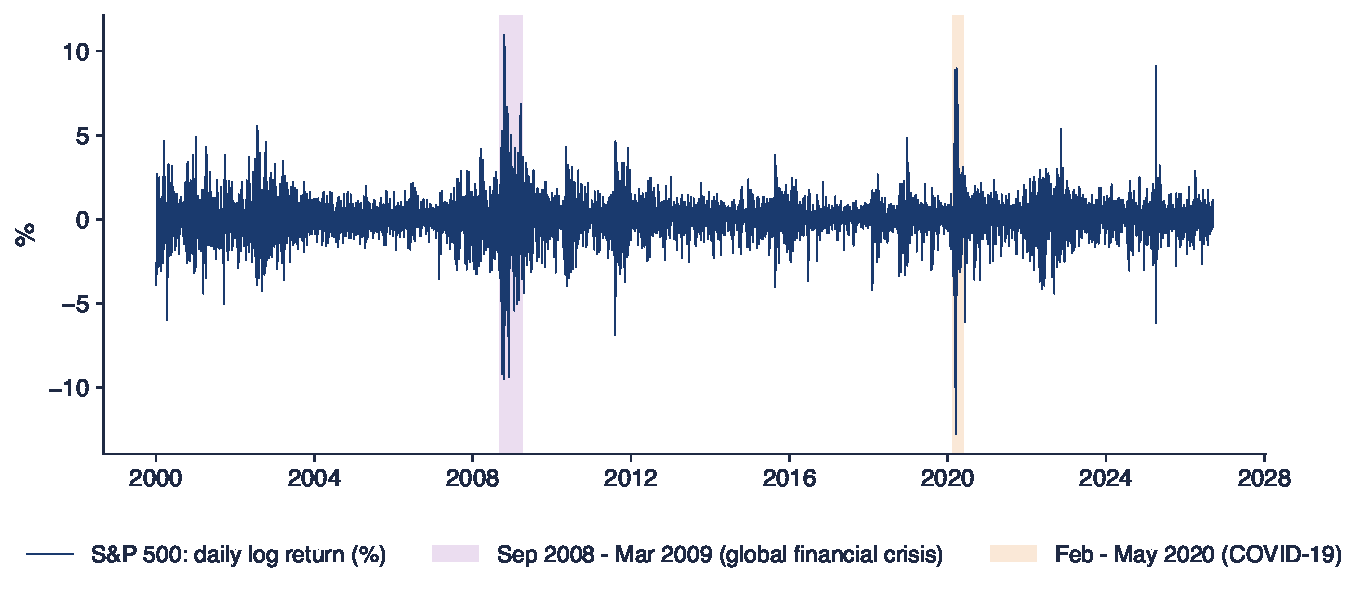
\includegraphics[width=0.97\textwidth,height=0.50\textheight,keepaspectratio]{sfm_ch9_returns.pdf}
\end{center}
\vspace{-0.25cm}
\begin{itemize}
    \item Randamente logaritmice zilnice $r_t = 100(\ln P_t - \ln P_{t-1})$, în \%, 6\,714 zile pînă la 18 septembrie 2026; cea mai mare scădere: $-12{,}8\%$ pe 16 martie 2020; cea mai mare creștere: $11{,}0\%$ pe 13 octombrie 2008
    \item Abaterea standard: $0{,}42\%$ în 2017, $3{,}52\%$ din septembrie 2008 pînă în martie 2009, $3{,}70\%$ din februarie pînă în mai 2020
    \item Variațiile mari urmează după variații mari, de orice semn: volatility clustering \refEngle
\end{itemize}
\sfmquantlet{Ch_09}{SFM_ch9_volatility_markets}
\end{frame}

\begin{frame}{Două crize: 2008 și 2020}
\itemsize{\footnotesize}
\begin{columns}[T]
\begin{column}{0.48\textwidth}
\centering
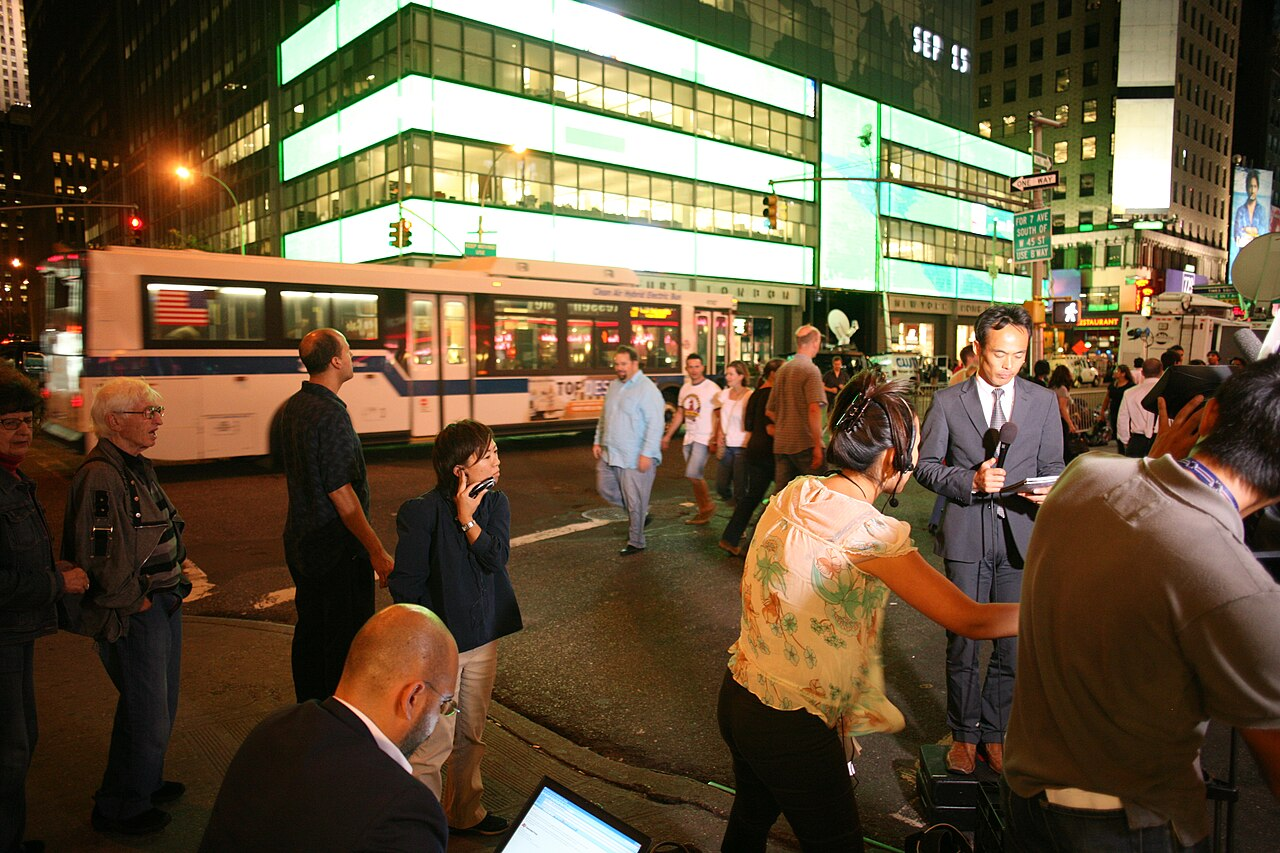
\includegraphics[height=0.30\textheight]{ch0_lehman_2008.jpg}\\[1mm]
\imgcap{Sediul Lehman Brothers, New York, 15 septembrie 2008}
\imgcredit{https://commons.wikimedia.org/wiki/File:Lehman_Brothers-NYC-20080915.jpg}{Foto: Robert Scoble (2008); CC BY 2.0; Wikimedia Commons}
\end{column}
\begin{column}{0.48\textwidth}
\centering
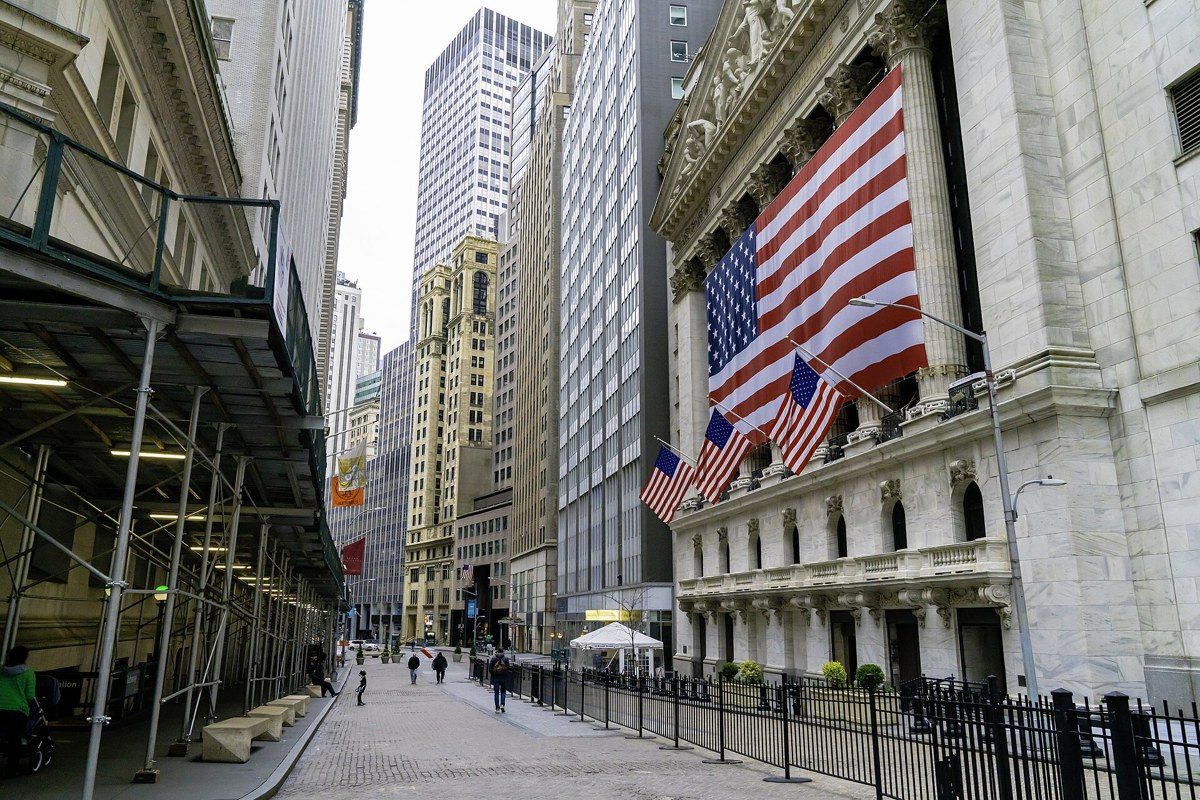
\includegraphics[height=0.30\textheight]{ch0_fidi_march_2020.jpg}\\[1mm]
\imgcap{Districtul financiar din New York, 25 martie 2020}
\imgcredit{https://commons.wikimedia.org/wiki/File:Subdued_FiDi_(50063555551).jpg}{Foto: Billie Grace Ward (2020); CC BY 2.0; Wikimedia Commons}
\end{column}
\end{columns}\begin{itemize}
    \item 15 septembrie 2008: Lehman Brothers intră în faliment; martie 2020: pandemia COVID-19 duce la închiderea economiilor
    \item În ambele episoade abaterea standard zilnică a S\&P 500 a fost de 8{,}3 și, respectiv, de 8{,}8 ori mai mare decît în 2017; calmul a revenit abia după cîteva luni
\end{itemize}
\end{frame}

\begin{frame}{Utilitatea modelării varianței condiționate}
\itemsize{\small}
\begin{itemize}
    \item \textbf{Managementul riscului}: VaR (value at risk, valoarea expusă la risc) și ES (expected shortfall) au nevoie de volatilitatea de mîine, nu de volatilitatea medie din ultimii 20 de ani
    \begin{itemize}
        \item un VaR cu varianță constantă este prea mare în anii liniștiți și prea mic în crize (\sfmchlink{https://danpele.github.io/SFM/RO/Cursuri/capitol10_var_es_backtesting.pdf}{Capitolul 10})
    \end{itemize}
    \item \textbf{Portofolii}: ponderile depind de varianțe și covarianțe, care se schimbă în timp
    \item \textbf{Derivate}: prețurile opțiunilor depind de volatilitatea așteptată pînă la scadență
    \item \textbf{Inferență}: testele și intervalele de încredere care presupun varianță constantă pot fi greșite
    \begin{itemize}
        \item de aceea \sfmchlink{https://danpele.github.io/SFM/RO/Cursuri/capitol7_piete_eficiente_mers_aleator_vr.pdf}{Capitolul 7} a avut nevoie de teste valide și în prezența heteroscedasticității
    \end{itemize}
\end{itemize}
\end{frame}

\begin{frame}{Faptele stilizate pe care un model de volatilitate trebuie să le reproducă}
\itemsize{\small}
\begin{itemize}
    \item \textbf{Volatility clustering}: ACF (autocorrelation function, funcția de autocorelație) a lui $r_t^2$ este pozitivă și scade lent (\sfmchlink{https://danpele.github.io/SFM/RO/Cursuri/capitol8_estimatori_volatilitate.pdf}{Capitolul 8})
    \begin{itemize}
        \item S\&P 500: autocorelația lui $r_t^2$ la lagul 1: $0{,}31$; la lagul 50: încă $0{,}053$
    \end{itemize}
    \item \textbf{Cozi groase}: coeficient de boltire peste 3, valoarea distribuției Normale (\sfmchlink{https://danpele.github.io/SFM/RO/Cursuri/capitol2_distributii_clasice_fapte_stilizate.pdf}{Capitolul 2})
    \begin{itemize}
        \item randamentele zilnice S\&P 500: coeficientul de boltire $13{,}7$
    \end{itemize}
    \item \textbf{Efectul de levier}: scăderile cresc volatilitatea mai mult decît creșterile de aceeași mărime \refChristie
    \item \textbf{Revenirea volatilității la medie}: după o perioadă turbulentă, volatilitatea revine la un nivel pe termen lung
    \item Aproape nicio autocorelație în $r_t$ însuși (\sfmchlink{https://danpele.github.io/SFM/RO/Cursuri/capitol7_piete_eficiente_mers_aleator_vr.pdf}{Capitolul 7})
\end{itemize}
\end{frame}


%=============================================================================
\section{Media condiționată și varianța condiționată}
%=============================================================================

\begin{frame}{Condiționarea pe trecut}
\itemsize{\small}
\begin{itemize}
    \item $\mathcal{F}_{t-1}$: informația disponibilă la sfîrșitul zilei $t-1$ (randamentele trecute)
    \begin{itemize}
        \item speranța condiționată $E[X \mid \mathcal{F}_{t-1}]$: cea mai bună prognoză a lui $X$, dată fiind informația trecută (\sfmchlink{https://danpele.github.io/SFM/RO/Cursuri/capitol4_probabilitate.pdf}{Capitolul 4})
    \end{itemize}
    \item \textbf{Media condiționată}: $\mu_t = E[r_t \mid \mathcal{F}_{t-1}]$
    \begin{itemize}
        \item \sfmchlink{https://danpele.github.io/SFM/RO/Cursuri/capitol7_piete_eficiente_mers_aleator_vr.pdf}{Capitolul 7}: pentru randamentele zilnice, $\mu_t$ este aproape constantă: $\mu_t = \mu$
    \end{itemize}
    \item \textbf{Varianța condiționată}: $\sigma_t^2 = \mathrm{Var}(r_t \mid \mathcal{F}_{t-1}) = E[(r_t - \mu_t)^2 \mid \mathcal{F}_{t-1}]$
    \begin{itemize}
        \item $\sigma_t$ este \textbf{volatilitatea condiționată}: cunoscută la $t-1$, se schimbă de la o zi la alta
        \item \textbf{heteroscedasticitate}: o varianță care nu este constantă
    \end{itemize}
\end{itemize}
\end{frame}

\begin{frame}{Descompunerea de bază}
\itemsize{\small}
\begin{itemize}
    \item Toate modelele din acest capitol au forma $r_t = \mu + \varepsilon_t$, \quad $\varepsilon_t = \sigma_t z_t$
    \begin{itemize}
        \item $z_t$: \textbf{inovațiile}, i.i.d.\ cu media 0 și varianța 1 (Normale, Student-t, \dots)
        \item $\varepsilon_t$: \textbf{șocul} (randamentul minus media lui); $\sigma_t$ depinde doar de trecut
    \end{itemize}
    \item Consecințe
    \begin{itemize}
        \item $E[\varepsilon_t \mid \mathcal{F}_{t-1}] = \sigma_t E[z_t] = 0$: șocurile sînt o diferență de martingal, deci sînt necorelate
        \item $\mathrm{Var}(\varepsilon_t \mid \mathcal{F}_{t-1}) = \sigma_t^2$: varianța este previzibilă
        \item $\varepsilon_t$ sînt necorelate, dar nu independente: $\varepsilon_t^2$ este corelat cu $\varepsilon_{t-1}^2$
    \end{itemize}
    \item În termenii \sfmchlink{https://danpele.github.io/SFM/RO/Cursuri/capitol7_piete_eficiente_mers_aleator_vr.pdf}{Capitolului 7}: RW1 (creșteri i.i.d.) este respinsă, RW3 (creșteri necorelate) rămîne valabilă
\end{itemize}
\end{frame}

\begin{frame}{Exemplu rezolvat: varianța condiționată și varianța necondiționată}
\itemsize{\small}
\begin{itemize}
    \item O piață are zile liniștite ($\sigma_t^2 = 0{,}5$) și zile agitate ($\sigma_t^2 = 4{,}5$), fiecare cu probabilitatea $1/2$; media este 0
    \begin{itemize}
        \item legea varianței totale: $\mathrm{Var}(r_t) = E[\mathrm{Var}(r_t \mid \mathcal{F}_{t-1})] + \mathrm{Var}(E[r_t \mid \mathcal{F}_{t-1}])$
        \item pas cu pas: $0{,}5 \times 0{,}5 + 0{,}5 \times 4{,}5 + 0 = 2{,}50$, deci abaterea standard necondiționată este $1{,}58\%$
    \end{itemize}
    \item Varianța necondiționată este o medie; varianța condiționată ne spune în ce fel de zi ne aflăm
    \begin{itemize}
        \item o zi liniștită: $\sigma_t = 0{,}71\%$; o zi agitată: $\sigma_t = 2{,}12\%$; media de $1{,}58\%$ nu descrie niciuna dintre ele
    \end{itemize}
    \item Un amestec de distribuții Normale cu varianțe diferite are cozi groase: heteroscedasticitatea condiționată creează boltire
\end{itemize}
\end{frame}


%=============================================================================
\section{Modelul ARCH}
%=============================================================================

\begin{frame}{1982: Robert Engle și modelul ARCH}
\itemsize{\footnotesize}
\begin{columns}[T]
\begin{column}{0.60\textwidth}
\begin{itemize}
    \item \refEngle: \textbf{ARCH} (autoregressive conditional heteroskedasticity, heteroscedasticitate condiționată autoregresivă): varianța de azi depinde de pătratele șocurilor de ieri
    \begin{itemize}
        \item prima aplicație: varianța inflației din Regatul Unit; scris în timpul vizitei lui Engle la London School of Economics
    \end{itemize}
    \item \href{https://www.nobelprize.org/prizes/economic-sciences/2003/summary/}{Premiul Nobel 2003}: „pentru metode de analiză a seriilor de timp economice cu volatilitate variabilă în timp (ARCH)”
    \begin{itemize}
        \item împărțit cu Clive Granger (cointegrare); prelegerea Nobel: \refEngleN
    \end{itemize}
\end{itemize}
\end{column}
\begin{column}{0.36\textwidth}
\centering

\includegraphics[height=0.25\textheight]{ch9_engle_2022.jpg}\\[1mm]
\imgcap{Robert F. Engle (2022)}
\imgcredit{https://commons.wikimedia.org/wiki/File:0603-Kraneshares_KRBN-RobertEngle-JonDemske-16_(cropped).jpg}{Foto: Jon Demske (2022); CC BY-SA 4.0; Wikimedia Commons}\\[1mm]
\centering
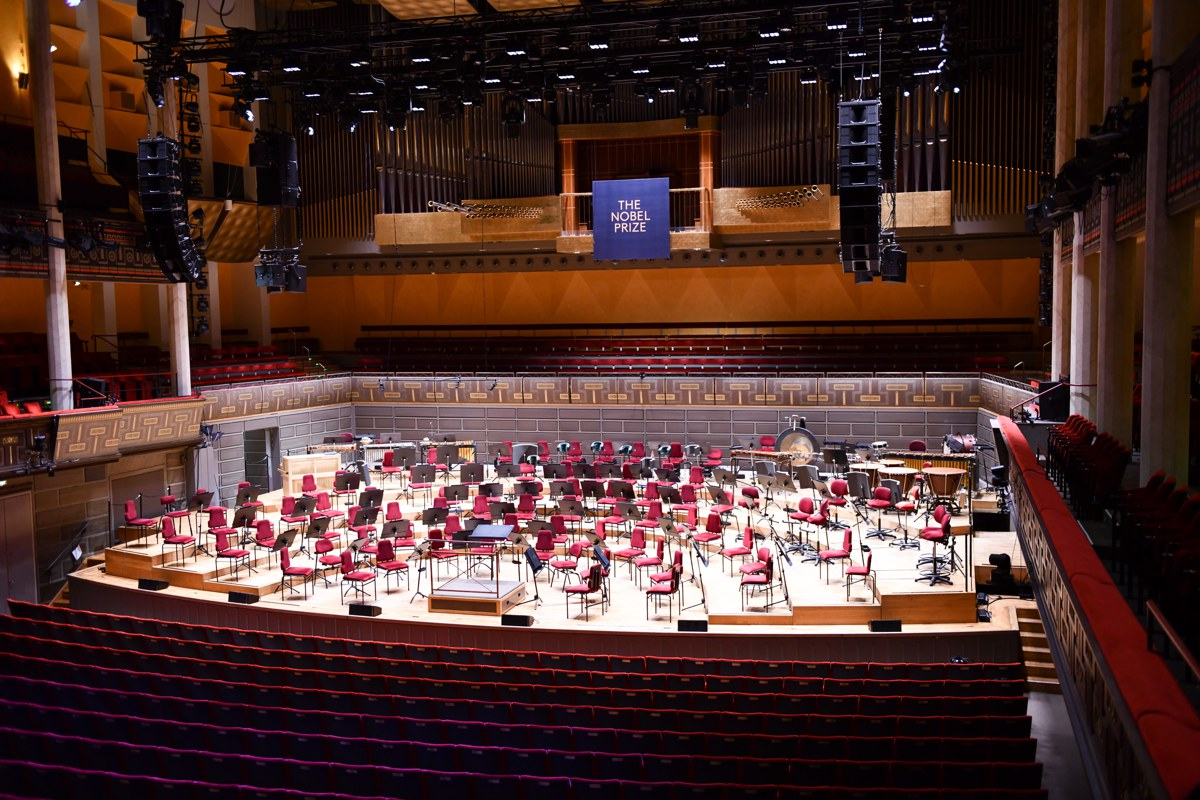
\includegraphics[height=0.16\textheight]{ch9_stockholm_concert_hall.jpg}\\[1mm]
\imgcap{Sala de concerte din Stockholm, unde se decernează Premiile Nobel}
\imgcredit{https://commons.wikimedia.org/wiki/File:Konserthuset_Stockholm_(Stockholm_Concert_Hall).jpg}{Foto: Karen Zhou (2025); CC BY-SA 4.0; Wikimedia Commons}
\end{column}
\end{columns}
\end{frame}

\begin{frame}{ARCH(1): definiție}
\itemsize{\small}
\begin{itemize}
    \item $\varepsilon_t = \sigma_t z_t$, \quad $\sigma_t^2 = \omega + \alpha\,\varepsilon_{t-1}^2$, \quad $\omega > 0$, $\alpha \ge 0$
    \begin{itemize}
        \item în cuvinte: varianța de azi = o constantă plus o fracțiune $\alpha$ din pătratul șocului de ieri
        \item $\omega$: varianța după un șoc nul; $\alpha$: reacția la șocul de ieri; restricțiile asigură o varianță pozitivă
        \item un șoc mare ieri, indiferent de semn, crește varianța de azi
    \end{itemize}
    \item „Autoregresiv”: $\varepsilon_t^2$ urmează un model AR(1) (autoregresiv)
    \begin{itemize}
        \item scriem $\varepsilon_t^2 = \sigma_t^2 + v_t$, cu $v_t = \sigma_t^2(z_t^2 - 1)$, $E[v_t \mid \mathcal{F}_{t-1}] = 0$
        \item atunci $\varepsilon_t^2 = \omega + \alpha\,\varepsilon_{t-1}^2 + v_t$: un AR(1) pentru pătratele șocurilor
    \end{itemize}
    \item De aici, ACF a lui $\varepsilon_t^2$ este $\rho(k) = \alpha^k$ cînd momentul de ordinul patru există: clustering, dar o scădere rapidă
\end{itemize}
\end{frame}

\begin{frame}{ARCH(1): proprietăți}
\itemsize{\small}
\begin{itemize}
    \item Media și autocorelația: $E[\varepsilon_t] = 0$, $\mathrm{Cov}(\varepsilon_t, \varepsilon_{t-k}) = 0$ pentru $k \ne 0$
    \item \textbf{Varianța necondiționată} (dacă $\alpha < 1$): aplicăm media în $\sigma_t^2 = \omega + \alpha\varepsilon_{t-1}^2$
    \begin{itemize}
        \item $\bar\sigma^2 = E[\varepsilon_t^2] = \omega + \alpha\bar\sigma^2$, deci $\bar\sigma^2 = \omega/(1 - \alpha)$
    \end{itemize}
    \item \textbf{Coeficientul de boltire} cu $z_t$ Normale (dacă $3\alpha^2 < 1$): $K = \dfrac{E[\varepsilon_t^4]}{(E[\varepsilon_t^2])^2} = 3\,\dfrac{1 - \alpha^2}{1 - 3\alpha^2} > 3$
    \begin{itemize}
        \item inovații Normale, dar randamente cu cozi groase \refFHH
        \item dacă $\alpha \ge 1/\sqrt{3} = 0{,}577$, momentul de ordinul patru este infinit
    \end{itemize}
    \item \textbf{Exemplu rezolvat}: $\omega = 0{,}5$, $\alpha = 0{,}5$
    \begin{itemize}
        \item $\bar\sigma^2 = 0{,}5/0{,}5 = 1{,}00$; $K = 3 \times 0{,}75/0{,}25 = 9{,}0$; după un șoc $\varepsilon_{t-1} = 2$: $\sigma_t^2 = 0{,}5 + 0{,}5 \times 4 = 2{,}50$, $\sigma_t = 1{,}58$
    \end{itemize}
\end{itemize}
\end{frame}

\begin{frame}{Traiectorii simulate: i.i.d., ARCH(1) și GARCH(1,1)}
\itemsize{\footnotesize}
\begin{center}
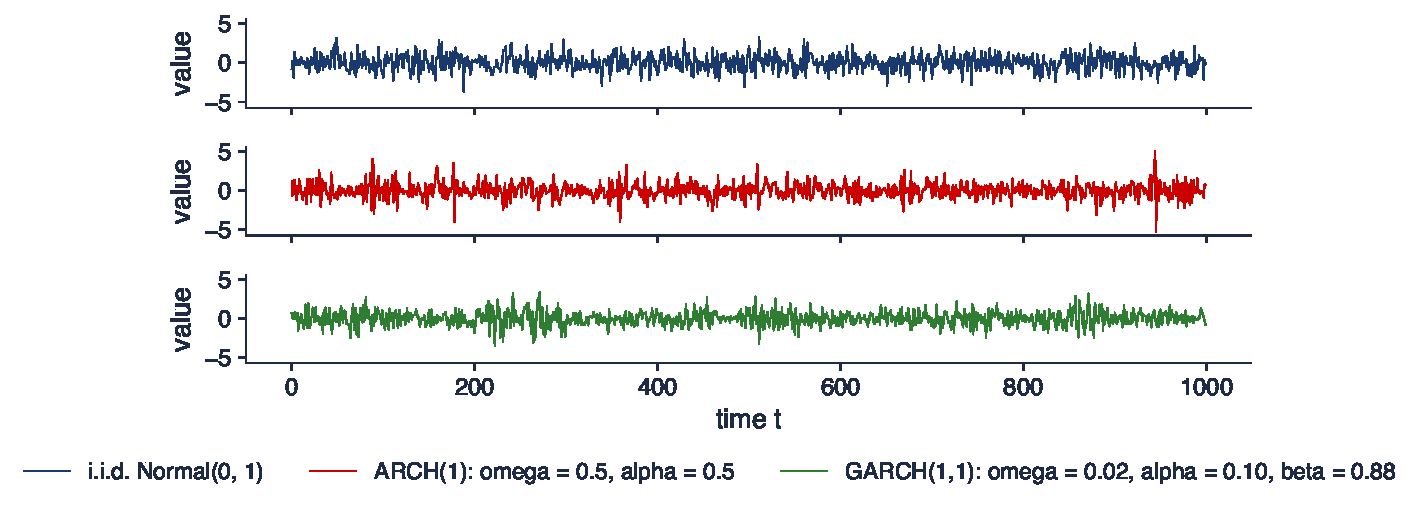
\includegraphics[width=0.97\textwidth,height=0.48\textheight,keepaspectratio]{sfm_ch9_simulated.pdf}
\end{center}
\vspace{-0.25cm}
\begin{itemize}
    \item Trei serii de 1000 de valori cu varianța necondiționată 1; ARCH(1) cu $\omega = \alpha = 0{,}5$, GARCH(1,1) cu $\omega = 0{,}02$, $\alpha = 0{,}10$, $\beta = 0{,}88$ (secțiunea următoare)
    \item Coeficientul de boltire de selecție: i.i.d.\ $3{,}12$, ARCH $4{,}91$, GARCH $3{,}74$; teoretic: 3, $9{,}0$, $6{,}06$; momentul de ordinul patru converge lent
    \item ARCH(1) produce vîrfuri izolate; GARCH(1,1) produce perioade lungi liniștite și perioade lungi agitate, ca în randamentele reale
\end{itemize}
\sfmquantlet{Ch_09}{SFM_ch9_simulation_likelihood}
\end{frame}

\begin{frame}{ARCH($q$) și limitele lui}
\itemsize{\footnotesize}
\begin{itemize}
    \item \textbf{ARCH($q$)}: $\sigma_t^2 = \omega + \alpha_1\varepsilon_{t-1}^2 + \dots + \alpha_q\varepsilon_{t-q}^2$, $\alpha_i \ge 0$; staționar dacă $\sum_i \alpha_i < 1$
    \begin{itemize}
        \item $q$: numărul de laguri; $\alpha_i$: reacția la șocul de acum $i$ zile
        \item efectul unui șoc durează exact $q$ zile; clustering-ul real durează luni
    \end{itemize}
    \item Testarea efectelor ARCH: testul ARCH-LM al lui Engle (regresia lui $\hat\varepsilon_t^2$ pe propriile laguri), \sfmchlink{https://danpele.github.io/SFM/RO/Cursuri/capitol8_estimatori_volatilitate.pdf}{Capitolul 8}
\end{itemize}\begin{center}
\footnotesize
\begin{tabular}{lrrrrr}
\toprule
S\&P 500, $z_t$ Normale & parametri & log-verosimilitate & AIC & BIC & $\sum\alpha_i$ (+$\beta$) \\
\midrule
ARCH(1) & 3 & $-10305{,}5$ & 20617{,}0 & 20637{,}5 & $0{,}394$ \\
ARCH(5) & 7 & $-9340{,}5$ & 18695{,}1 & 18742{,}7 & $0{,}816$ \\
ARCH(10) & 12 & $-9227{,}6$ & 18479{,}3 & 18561{,}0 & $0{,}849$ \\
GARCH(1,1) & 4 & $-9218{,}0$ & \textbf{18444{,}0} & \textbf{18471{,}2} & $0{,}980$ \\
\bottomrule
\end{tabular}
\end{center}
\begin{itemize}
    \item Interpretare: ARCH are nevoie de zece laguri și rămîne totuși inferior modelului GARCH(1,1), care are patru parametri (AIC și BIC: valoarea mai mică este mai bună, secțiunea 10)
\end{itemize}\sfmquantlet{Ch_09}{SFM_ch9_garch_estimation}
\end{frame}


%=============================================================================
\section{Modelul GARCH(1,1)}
%=============================================================================

\begin{frame}{1986: Tim Bollerslev și modelul GARCH}
\itemsize{\small}
\begin{columns}[T]
\begin{column}{0.56\textwidth}
\begin{itemize}
    \item \refBoll, doctorand al lui Engle la University of California, San Diego: adaugă în ecuație varianța de ieri
    \begin{itemize}
        \item \textbf{GARCH} (generalised ARCH, ARCH generalizat): cîțiva parametri înlocuiesc un ARCH($q$) lung
    \end{itemize}
    \item Inovații Student-t pentru randamente: \refBollT
    \item GARCH(1,1) rămîne modelul de referință: \refHL{} au comparat 330 de modele și l-au găsit greu de întrecut la cursurile de schimb
\end{itemize}
\end{column}
\begin{column}{0.40\textwidth}
\centering
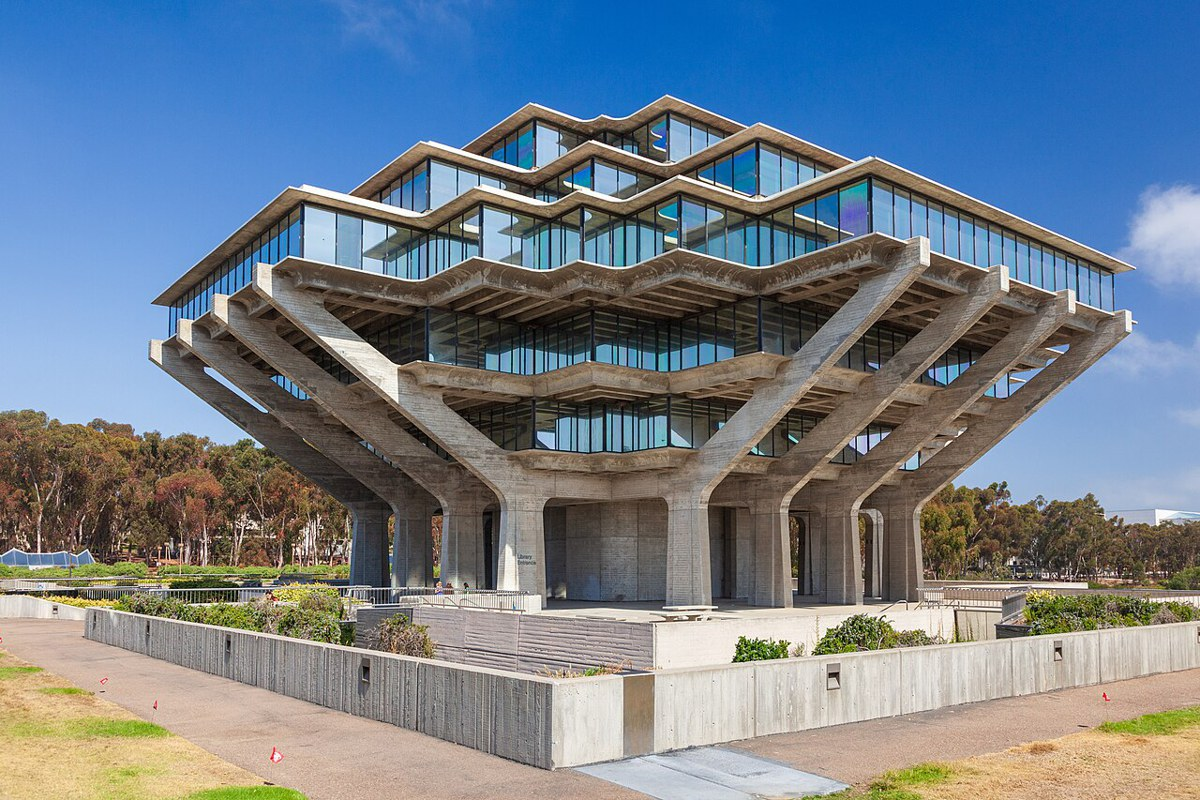
\includegraphics[height=0.36\textheight]{ch9_ucsd_geisel_2010.jpg}\\[1mm]
\imgcap{Biblioteca Geisel, University of California, San Diego}
\imgcredit{https://commons.wikimedia.org/wiki/File:Geisel_Library,_UC_San_Diego.jpg}{Foto: Stephen Bay (2010); CC BY 4.0; Wikimedia Commons}
\end{column}
\end{columns}
\end{frame}

\begin{frame}{GARCH(1,1): definiție}
\itemsize{\small}
\begin{itemize}
    \item $r_t = \mu + \varepsilon_t$, \quad $\varepsilon_t = \sigma_t z_t$, \quad $\sigma_t^2 = \omega + \alpha\,\varepsilon_{t-1}^2 + \beta\,\sigma_{t-1}^2$
    \begin{itemize}
        \item $\omega > 0$, $\alpha \ge 0$, $\beta \ge 0$: varianța rămîne pozitivă
    \end{itemize}
    \item Interpretarea parametrilor
    \begin{itemize}
        \item $\alpha$: \textbf{reacția} la știrile de ieri (mărimea saltului după un șoc)
        \item $\beta$: \textbf{memoria} varianței (cît din nivelul de ieri se păstrează)
        \item $\alpha + \beta$: \textbf{persistența}; $\omega$ fixează nivelul pe termen lung
    \end{itemize}
    \item Prin recurență, un ARCH($\infty$) cu ponderi geometrice
    \begin{itemize}
        \item $\sigma_t^2 = \dfrac{\omega}{1 - \beta} + \alpha\sum_{j=0}^{\infty}\beta^j\,\varepsilon_{t-1-j}^2$: toate șocurile trecute contează, cu ponderi descrescătoare
        \item șocul de acum $j + 1$ zile primește ponderea $\alpha\beta^j$
    \end{itemize}
\end{itemize}
\end{frame}

\begin{frame}{Staționaritate, varianța pe termen lung și boltire}
\itemsize{\small}
\begin{itemize}
    \item Ca la ARCH: $\varepsilon_t^2 = \omega + (\alpha + \beta)\varepsilon_{t-1}^2 + v_t - \beta v_{t-1}$, un ARMA(1,1) pentru pătratele șocurilor
    \begin{itemize}
        \item $v_t = \varepsilon_t^2 - \sigma_t^2$: surpriza din pătratul șocului, ca la ARCH(1)
        \item ARMA: model autoregresiv cu medie mobilă; ACF a lui $\varepsilon_t^2$ scade ca $(\alpha + \beta)^k$ la lagul $k$
    \end{itemize}
    \item \textbf{Staționar în covarianță} dacă $\alpha + \beta < 1$; atunci \textbf{varianța necondiționată (pe termen lung)} este
    \begin{itemize}
        \item $\bar\sigma^2 = E[\sigma_t^2] = \dfrac{\omega}{1 - \alpha - \beta}$, \quad volatilitatea anualizată $\sqrt{252\,\bar\sigma^2}$ pentru 252 de zile de tranzacționare
    \end{itemize}
    \item Coeficientul de boltire cu $z_t$ Normale, dacă $(\alpha + \beta)^2 + 2\alpha^2 < 1$: $K = 3\,\dfrac{1 - (\alpha + \beta)^2}{1 - (\alpha + \beta)^2 - 2\alpha^2} > 3$
    \begin{itemize}
        \item $\alpha = 0{,}10$, $\beta = 0{,}88$: $(\alpha + \beta)^2 + 2\alpha^2 = 0{,}9804$, $K = 6{,}06$
    \end{itemize}
\end{itemize}
\end{frame}

\begin{frame}{Persistența și timpul de înjumătățire}
\itemsize{\small}
\begin{itemize}
    \item Prognoza varianței peste $h$ zile (derivată în secțiunea 11): $E[\sigma_{t+h}^2 \mid \mathcal{F}_t] - \bar\sigma^2 = (\alpha + \beta)^{h-1}(\sigma_{t+1}^2 - \bar\sigma^2)$
    \begin{itemize}
        \item $E[\cdot \mid \mathcal{F}_t]$: prognoza făcută la sfîrșitul zilei $t$; $\bar\sigma^2$: varianța pe termen lung
        \item o abatere de la varianța pe termen lung se micșorează cu factorul $\alpha + \beta$ în fiecare zi
    \end{itemize}
    \item \textbf{Timpul de înjumătățire}: numărul de zile după care a dispărut jumătate dintr-un șoc de varianță
    \begin{itemize}
        \item $(\alpha + \beta)^{h} = 1/2 \;\Rightarrow\; h_{1/2} = \dfrac{\ln 0{,}5}{\ln(\alpha + \beta)}$
        \item $\alpha + \beta = 0{,}90$: 6{,}6 zile; $0{,}98$: 34{,}3 zile; $0{,}99$: 69{,}0 zile: schimbările mici în apropiere de 1 contează mult
    \end{itemize}
    \item Randamentele zilnice ale acțiunilor: $\alpha$ în jur de 0,05--0,15, $\beta$ în jur de 0,80--0,93, $\alpha + \beta$ apropiat de 1 (secțiunea 7)
\end{itemize}
\end{frame}

\begin{frame}{Exemplu rezolvat: un pas GARCH(1,1)}
\itemsize{\small}
\begin{itemize}
    \item Randamente zilnice în \%: $\omega = 0{,}02$, $\alpha = 0{,}10$, $\beta = 0{,}88$, $\mu = 0$
    \item Mărimile pe termen lung
    \begin{itemize}
        \item persistența $\alpha + \beta = 0{,}98$; $\bar\sigma^2 = 0{,}02/(1 - 0{,}98) = 1{,}00$; volatilitatea anualizată $\sqrt{252 \times 1{,}00} = 15{,}9\%$
        \item timpul de înjumătățire $\ln 0{,}5/\ln 0{,}98 = 34{,}3$ zile
    \end{itemize}
    \item Azi: $\sigma_t^2 = 1{,}2$, iar randamentul este $r_t = -3\%$
    \begin{itemize}
        \item mîine: $\sigma_{t+1}^2 = 0{,}02 + 0{,}10 \times 9 + 0{,}88 \times 1{,}2 = 1{,}976$, $\sigma_{t+1} = 1{,}41\%$
        \item șocul a crescut varianța de la 1,2 la aproape 2; apoi ea scade spre 1{,}00 cu factorul 0{,}98 pe zi
    \end{itemize}
\end{itemize}
\end{frame}

\begin{frame}{IGARCH și legătura cu EWMA}
\itemsize{\small}
\begin{itemize}
    \item \textbf{IGARCH} (integrated GARCH, GARCH integrat) \refEB: $\alpha + \beta = 1$
    \begin{itemize}
        \item șocurile varianței nu se sting niciodată: nu există timp de înjumătățire și nici varianță necondiționată finită
        \item prognoza varianței este aceeași pentru orice orizont
    \end{itemize}
    \item \textbf{EWMA} (exponentially weighted moving average, \sfmchlink{https://danpele.github.io/SFM/RO/Cursuri/capitol8_estimatori_volatilitate.pdf}{Capitolul 8}): $\sigma_t^2 = \lambda\sigma_{t-1}^2 + (1 - \lambda)r_{t-1}^2$
    \begin{itemize}
        \item este un IGARCH cu $\omega = 0$, $\alpha = 1 - \lambda$, $\beta = \lambda$; RiskMetrics folosește $\lambda = 0{,}94$ pentru date zilnice
        \item EWMA: nimic de estimat, dar fără revenire la medie; GARCH: trei parametri, iar volatilitatea revine la $\bar\sigma$
    \end{itemize}
    \item \textbf{Întrebare pentru sală}: un analist prognozează volatilitatea peste un an cu EWMA imediat după un crah. Unde greșește?
    \begin{itemize}
        \item \textbf{Răspuns}: EWMA păstrează nivelul de criză de azi pentru tot anul; GARCH îl lasă să scadă spre nivelul pe termen lung
    \end{itemize}
\end{itemize}
\end{frame}


%=============================================================================
\section{Estimarea prin verosimilitate maximă}
%=============================================================================

\begin{frame}{Verosimilitatea unui model GARCH}
\itemsize{\small}
\begin{itemize}
    \item Randamentele sînt dependente, deci descompunem densitatea comună în densități condiționate
    \begin{itemize}
        \item $f$: o densitate de probabilitate; $T$: numărul de randamente; $\theta$: vectorul parametrilor; $\ell$: log-verosimilitatea
        \item $f(r_1, \dots, r_T) = f(r_1)\prod_{t=2}^{T} f(r_t \mid \mathcal{F}_{t-1})$, iar $r_t \mid \mathcal{F}_{t-1} \sim N(\mu, \sigma_t^2)$ pentru inovații Normale
    \end{itemize}
    \item \textbf{Log-verosimilitatea condiționată}, cu $\theta = (\mu, \omega, \alpha, \beta)$:
    \begin{itemize}
        \item $\ell(\theta) = -\dfrac12\sum_{t=2}^{T}\Big[\ln(2\pi) + \ln\sigma_t^2(\theta) + \dfrac{(r_t - \mu)^2}{\sigma_t^2(\theta)}\Big]$
        \item în cuvinte: fiecare zi adaugă o penalizare pentru un $\sigma_t^2$ mare și una pentru o eroare la pătrat mare în raport cu $\sigma_t^2$
        \item $\sigma_t^2(\theta)$ se calculează recursiv, pornind de la o valoare inițială $\sigma_1^2$ (de exemplu, varianța de selecție)
    \end{itemize}
    \item \textbf{MLE} (maximum likelihood estimation, estimarea prin verosimilitate maximă): $\hat\theta = \arg\max_\theta \ell(\theta)$, cu $\omega > 0$, $\alpha, \beta \ge 0$, $\alpha + \beta < 1$
    \begin{itemize}
        \item nu există o formulă explicită: un algoritm numeric de optimizare caută maximul \refFHH
    \end{itemize}
\end{itemize}
\end{frame}

\begin{frame}{Verosimilitatea modelului ARCH(1)}
\itemsize{\footnotesize}
\begin{center}
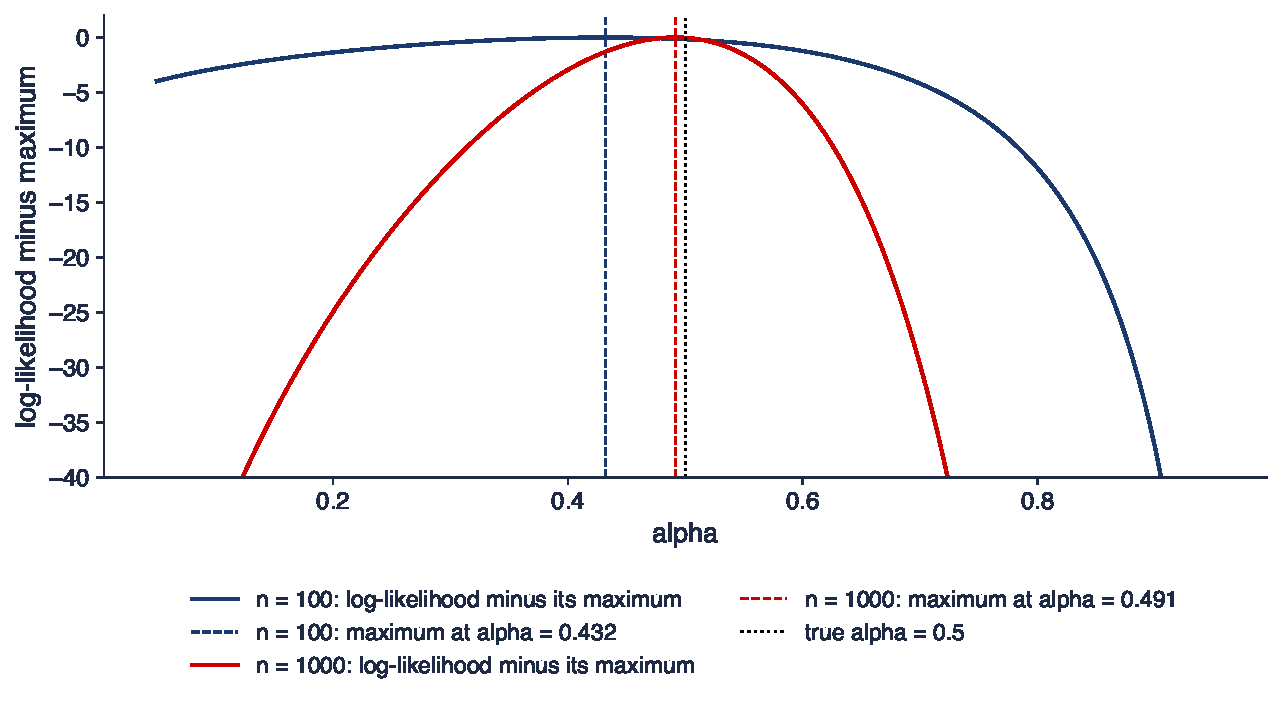
\includegraphics[width=0.97\textwidth,height=0.50\textheight,keepaspectratio]{sfm_ch9_lik_arch1.pdf}
\end{center}
\vspace{-0.25cm}
\begin{itemize}
    \item ARCH(1) simulat cu $\omega = \alpha = 0{,}5$; $\ell(\alpha)$ cu $\omega = 1 - \alpha$, ca în SFElikarch1; fiecare curbă minus maximul ei
    \item $n = 100$: $\hat\alpha = 0{,}432$ (eroarea standard $0{,}127$); $n = 1000$: $\hat\alpha = 0{,}491$ ($0{,}035$)
    \item Interpretare: mai multe date fac curba mai ascuțită; curbura ei în punctul de maxim dă eroarea standard
\end{itemize}
\sfmquantlet{Ch_09}{SFM_ch9_simulation_likelihood}
\end{frame}

\begin{frame}{Verosimilitatea modelului GARCH(1,1)}
\itemsize{\footnotesize}
\begin{center}
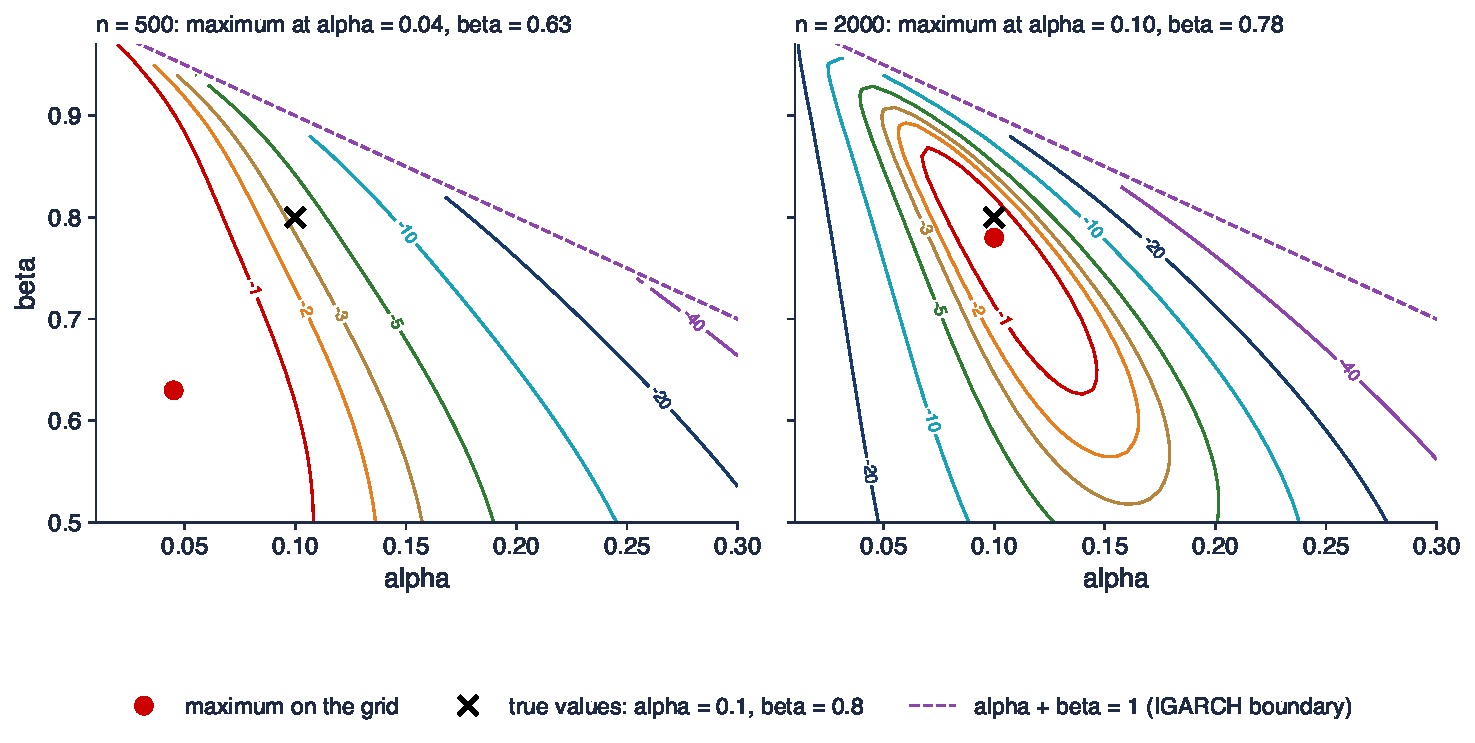
\includegraphics[width=0.97\textwidth,height=0.48\textheight,keepaspectratio]{sfm_ch9_lik_garch.pdf}
\end{center}
\vspace{-0.25cm}
\begin{itemize}
    \item GARCH(1,1) simulat, $\omega = 0{,}1$, $\alpha = 0{,}1$, $\beta = 0{,}8$; $\omega$ fixat astfel încît varianța necondiționată să fie egală cu varianța de selecție, ca în SFElikgarch; contururi: log-verosimilitatea minus maximul ei
    \item $n = 500$: maximul în $(0{,}04; 0{,}63)$, departe de valorile adevărate; $n = 2000$: $(0{,}10; 0{,}78)$
    \item Interpretare: o creastă lungă și plată, de-a lungul căreia $\alpha$ și $\beta$ se compensează: GARCH are nevoie de eșantioane lungi
\end{itemize}
\sfmquantlet{Ch_09}{SFM_ch9_simulation_likelihood}
\end{frame}

\begin{frame}{Estimarea pas cu pas și cu un pachet}
\itemsize{\footnotesize}
\begin{center}
\footnotesize
\begin{tabular}{lrrrr}
\toprule
S\&P 500, GARCH(1,1)-N & pas cu pas (SE) & \texttt{arch} & SE clasică & SE robustă \\
\midrule
$\mu$ & $0{,}0614$ ($0{,}0098$) & $0{,}0615$ & $0{,}0098$ & $0{,}0100$ \\
$\omega$ & $0{,}0253$ ($0{,}0030$) & $0{,}0254$ & $0{,}0030$ & $0{,}0048$ \\
$\alpha$ & $0{,}1205$ ($0{,}0086$) & $0{,}1206$ & $0{,}0086$ & $0{,}0118$ \\
$\beta$ & $0{,}8600$ ($0{,}0091$) & $0{,}8599$ & $0{,}0091$ & $0{,}0125$ \\
\bottomrule
\end{tabular}
\end{center}
\begin{itemize}
    \item Pas cu pas: scriem $-\ell(\theta)$ în Python și o minimizăm cu \texttt{scipy.optimize.minimize}, cu restricția $\alpha + \beta < 1$
    \begin{itemize}
        \item cele două variante diferă doar prin valoarea inițială a lui $\sigma_t^2$ și prin algoritmul de optimizare; log-verosimilitatea $-9219{,}9$ față de $-9218{,}0$
    \end{itemize}
    \item SE (standard error, eroarea standard) clasică: din inversa matricei hessiene (curbura lui $\ell$); robustă: validă și cînd $z_t$ nu este Normal \refBW
    \item Interpretare: SE robuste sînt de circa 1{,}4 ori mai mari (1{,}6 pentru $\omega$): cînd $z_t$ are cozi groase, SE clasice supraestimează precizia
\end{itemize}\sfmquantlet{Ch_09}{SFM_ch9_garch_estimation}
\end{frame}

\begin{frame}{Cvasi-verosimilitatea maximă}
\itemsize{\small}
\begin{itemize}
    \item \textbf{QMLE} (quasi-maximum likelihood estimation, estimarea prin cvasi-verosimilitate maximă): maximizăm verosimilitatea Normală chiar dacă $z_t$ nu este Normal
    \begin{itemize}
        \item estimările rămîn consistente dacă $\mu$ și $\sigma_t^2$ sînt corect specificate \refBW
        \item dar SE clasice sînt greșite: folosim SE robuste (de tip „sandwich”)
    \end{itemize}
    \item Reguli practice
    \begin{itemize}
        \item raportăm SE robuste (opțiunea implicită în \texttt{arch})
        \item folosim cel puțin 1000--2000 de observații zilnice; randamentele în \% evită problemele numerice cauzate de un $\omega$ foarte mic
        \item o estimare pe frontieră ($\alpha + \beta = 1$) nu are o eroare standard obișnuită: o raportăm ca IGARCH
    \end{itemize}
    \item O distribuție mai potrivită a inovațiilor dă estimări mai eficiente: secțiunea următoare
\end{itemize}
\end{frame}


%=============================================================================
\section{Inovații cu cozi groase}
%=============================================================================

\begin{frame}{Inovații Student-t și t asimetrice}
\itemsize{\small}
\begin{itemize}
    \item GARCH cu $z_t$ Normale explică doar o parte din boltire: randamentele S\&P 500 au $13{,}7$, reziduurile standardizate $\hat z_t = \hat\varepsilon_t/\hat\sigma_t$ au $4{,}7$
    \begin{itemize}
        \item cozile groase rămase trebuie să vină din distribuția lui $z_t$
    \end{itemize}
    \item \textbf{Student-t standardizată} cu $\nu > 2$ grade de libertate (\sfmchlink{https://danpele.github.io/SFM/RO/Cursuri/capitol2_distributii_clasice_fapte_stilizate.pdf}{Capitolul 2}) \refBollT
    \begin{itemize}
        \item $t_\nu$: o variabilă Student-t cu $\nu$ grade de libertate; $z_t = t_\nu\sqrt{(\nu - 2)/\nu}$ are varianța 1
        \item un $\nu$ mic înseamnă cozi groase: coeficientul de boltire $3 + 6/(\nu - 4)$ pentru $\nu > 4$; $\nu \to \infty$: distribuția Normală
        \item $\nu$ se estimează împreună cu $(\mu, \omega, \alpha, \beta)$
    \end{itemize}
    \item \textbf{t asimetrică} \refHansen: încă un parametru $\lambda \in (-1, 1)$; $\lambda < 0$: o coadă stîngă mai lungă
    \begin{itemize}
        \item modele incluse unul în altul: Normal $\subset$ t $\subset$ t asimetrică; le comparăm prin teste ale raportului de verosimilitate sau prin AIC/BIC (\sfmchlink{https://danpele.github.io/SFM/RO/Cursuri/capitol6_selectia_modelului_managementul_riscului.pdf}{Capitolul 6})
    \end{itemize}
\end{itemize}
\end{frame}

\begin{frame}{S\&P 500: trei distribuții ale inovațiilor}
\itemsize{\footnotesize}
\begin{center}
\footnotesize
\begin{tabular}{lrrrrrrr}
\toprule
GARCH(1,1) & $\omega$ & $\alpha$ & $\beta$ & $\nu$ & $\lambda$ & log-verosim. & $\alpha + \beta$ \\
\midrule
Normală & $0{,}0254$ & $0{,}121$ & $0{,}860$ & -- & -- & $-9218{,}0$ & $0{,}980$ \\
Student-t & $0{,}0157$ & $0{,}123$ & $0{,}872$ & $6{,}26$ & -- & $-9062{,}5$ & $0{,}995$ \\
t asimetrică & $0{,}0153$ & $0{,}120$ & $0{,}872$ & $6{,}92$ & $-0{,}114$ & $-9038{,}4$ & $0{,}993$ \\
\bottomrule
\end{tabular}
\end{center}
\begin{itemize}
    \item Statistica raportului de verosimilitate $2(\ell_1 - \ell_0)$ ($\ell_1$, $\ell_0$: log-verosimilitățile maxime ale modelului mai mare și ale celui mai mic): t față de Normal $311{,}0$ (o restricție, $\chi^2_{0{,}95}(1) = 3{,}84$); t asimetrică față de t $48{,}1$: ambele resping modelul mai mic
    \item $\hat\nu = 6{,}26$: cozi mult mai groase decît la distribuția Normală; $\hat\lambda = -0{,}114$: scăderile mari sînt mai frecvente decît creșterile mari
    \item Interpretare: $\alpha$ și $\beta$ aproape nu se schimbă; distribuția inovațiilor contează pentru cuantilele din coadă (VaR), mai puțin pentru $\sigma_t$
\end{itemize}\sfmquantlet{Ch_09}{SFM_ch9_garch_estimation}
\end{frame}

\begin{frame}{Graficele QQ ale reziduurilor standardizate}
\itemsize{\footnotesize}
\begin{center}
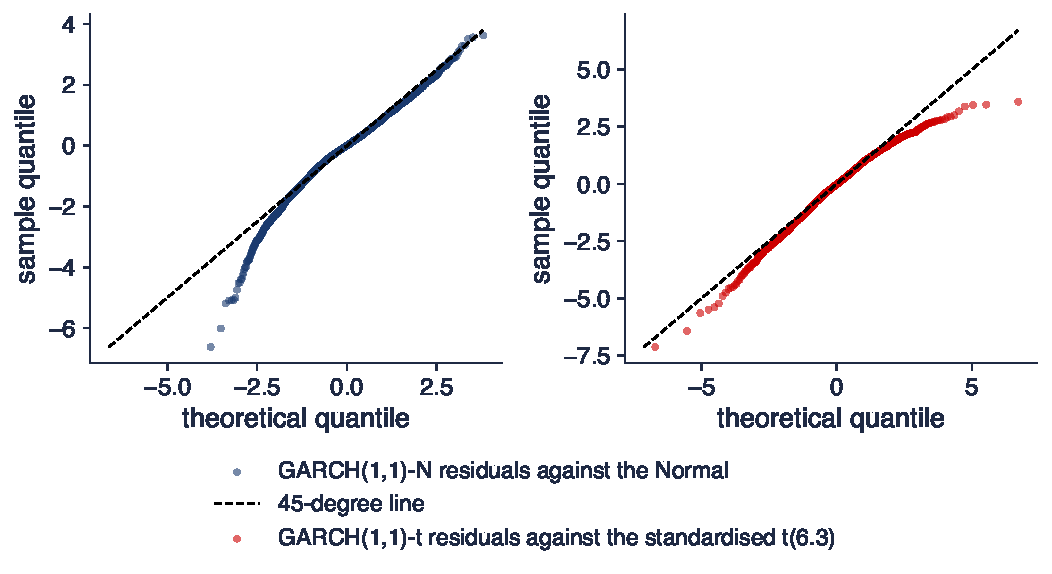
\includegraphics[width=0.97\textwidth,height=0.50\textheight,keepaspectratio]{sfm_ch9_qq.pdf}
\end{center}
\vspace{-0.25cm}
\begin{itemize}
    \item Stînga: reziduurile modelului GARCH cu inovații Normale față de distribuția Normală: cuantila de 0,1\% este $-4{,}81$, față de $-3{,}09$ teoretic
    \item Dreapta: reziduurile GARCH-t față de t standardizată cu $\hat\nu = 6{,}3$: $-4{,}79$ față de $-4{,}19$, mult mai aproape; cele mai mari scăderi rămîn mai adînci
    \item Interpretare: problema este coada stîngă: un motiv pentru inovații asimetrice și pentru modele asimetrice (secțiunea 8)
\end{itemize}
\sfmquantlet{Ch_09}{SFM_ch9_garch_estimation}
\end{frame}


%=============================================================================
\section{GARCH pe șase piețe}
%=============================================================================

\begin{frame}{Estimările GARCH(1,1)-t}
\itemsize{\footnotesize}
\begin{center}
\scriptsize
\begin{tabular}{lrrrrrrrr}
\toprule
& din & $\alpha$ & $\beta$ & $\nu$ & $\alpha + \beta$ & înjumătățire & vol. termen lung & vol. selecție \\
\midrule
S\&P 500 & 2000 & $0{,}123$ & $0{,}872$ & $6{,}26$ & $0{,}995$ & 131 & 27{,}3 & 19{,}2 \\
DAX & 2000 & $0{,}097$ & $0{,}895$ & $7{,}08$ & $0{,}992$ & 88 & 25{,}9 & 22{,}4 \\
BET & 2000 & $0{,}192$ & $0{,}799$ & $5{,}01$ & $0{,}991$ & 74 & 34{,}7 & 22{,}1 \\
Bitcoin & 2014 & $0{,}109$ & $0{,}891$ & $3{,}18$ & $1{,}000$ & -- & -- & 66{,}6 \\
TLV & 2010 & $0{,}139$ & $0{,}824$ & $4{,}91$ & $0{,}963$ & 18 & 28{,}2 & 26{,}5 \\
SNP & 2010 & $0{,}135$ & $0{,}807$ & $4{,}81$ & $0{,}942$ & 12 & 25{,}6 & 24{,}5 \\
\bottomrule
\end{tabular}
\end{center}
\begin{itemize}
    \item Randamente logaritmice zilnice în \% pînă la 18 septembrie 2026; SE robuste pentru $\hat\alpha$ și $\hat\beta$ între 0{,}010 și 0{,}041; timpul de înjumătățire în zile; volatilitățile anualizate cu numărul efectiv de observații pe an, în \%
    \item Indicii: $\alpha + \beta$ între 0{,}991 și 0{,}995, timpi de înjumătățire de 74--131 de zile de tranzacționare; acțiunile BVB: memorie mai scurtă (TLV 18 zile, SNP 12 zile)
    \item BET: cel mai mare $\alpha$ (0{,}192): o reacție mai puternică la știri; toate valorile $\hat\nu$ sînt între 3{,}2 și 7{,}1: cozi groase peste tot
\end{itemize}\sfmquantlet{Ch_09}{SFM_ch9_volatility_markets}
\end{frame}

\begin{frame}{Interpretarea rezultatelor: Bitcoin și volatilitatea pe termen lung}
\itemsize{\small}
\begin{itemize}
    \item Bitcoin: $\hat\alpha + \hat\beta = 1{,}0000$, pe frontiera $\alpha + \beta < 1$: un IGARCH
    \begin{itemize}
        \item nu există timp de înjumătățire și nici volatilitate pe termen lung: modelul se comportă ca un EWMA cu $\lambda \approx 0{,}891$
        \item $\hat\nu = 3{,}18$: cozi extrem de groase (momentul de ordinul patru al lui $z_t$ nu există)
    \end{itemize}
    \item \textbf{Întrebare pentru sală}: S\&P 500: volatilitatea pe termen lung 27{,}3\%, volatilitatea de selecție 19{,}2\%. Este greșit modelul?
    \begin{itemize}
        \item \textbf{Răspuns}: nu neapărat: $\bar\sigma^2 = \omega/(1 - \alpha - \beta)$ se împarte la $1 - \alpha - \beta = 0{,}0053$, un număr mic și imprecis
        \item GARCH cu inovații Normale dă 18{,}1\%; nivelul pe termen lung este cel mai puțin sigur rezultat al unui GARCH persistent
    \end{itemize}
\end{itemize}
\end{frame}

\begin{frame}{Volatilitatea condiționată: S\&P 500 și DAX}
\itemsize{\footnotesize}
\begin{center}
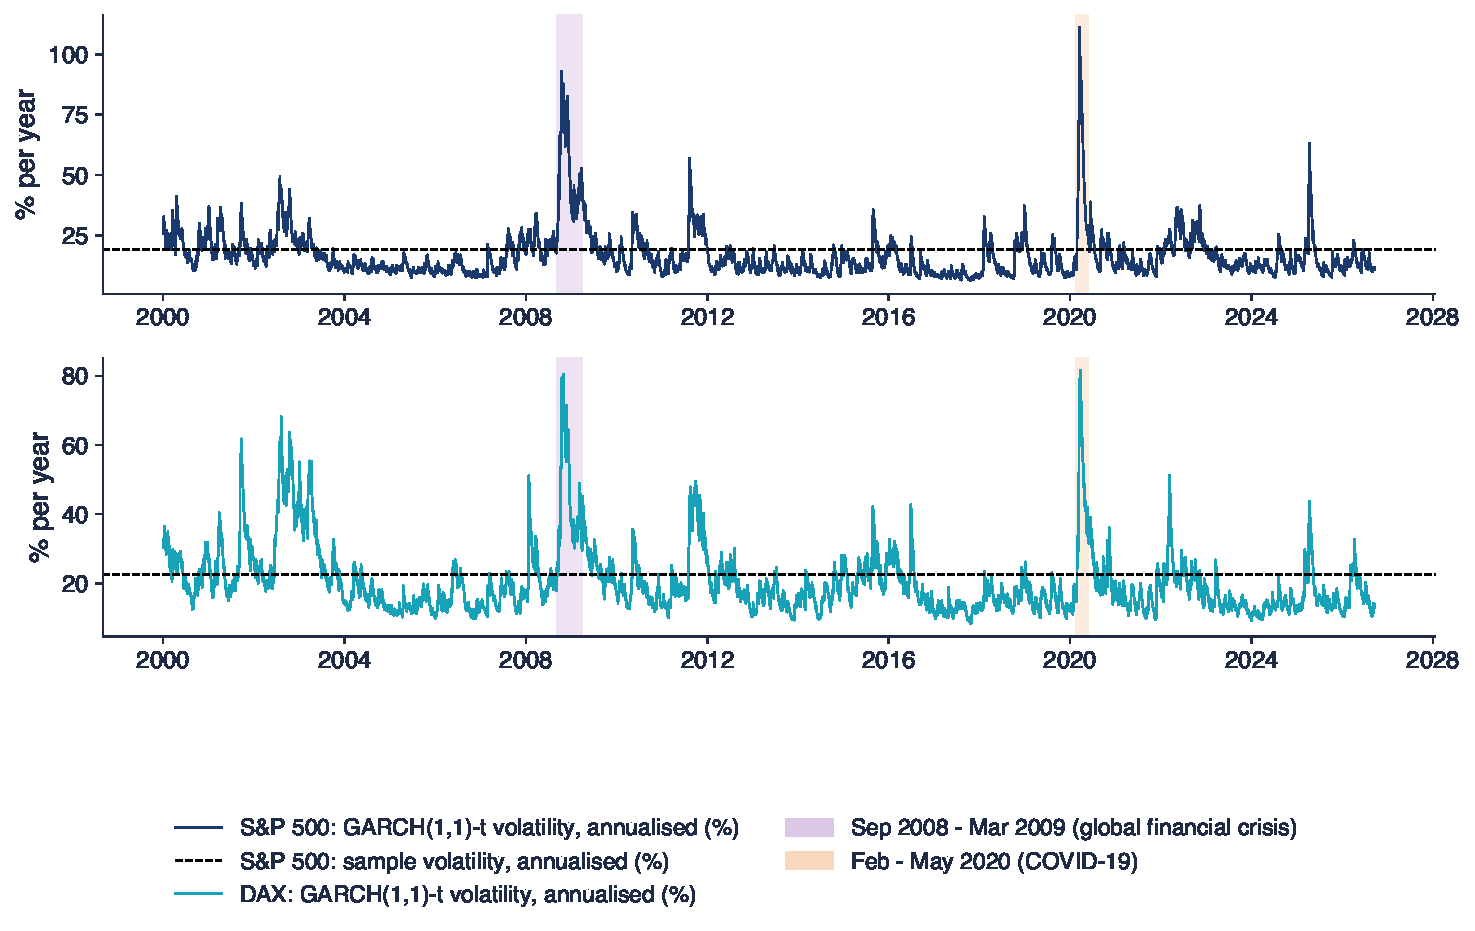
\includegraphics[width=0.97\textwidth,height=0.56\textheight,keepaspectratio]{sfm_ch9_vol_sp500_dax.pdf}
\end{center}
\vspace{-0.25cm}
\begin{itemize}
    \item Volatilitatea GARCH(1,1)-t $\hat\sigma_t$, anualizată, ca în SFEvolgarchest; linia întreruptă: volatilitatea de selecție
    \item S\&P 500: vîrfuri de 93\% (16 octombrie 2008) și 111\% (17 martie 2020); mediana 14\%; la 18 septembrie 2026: 12\%
\end{itemize}
\sfmquantlet{Ch_09}{SFM_ch9_volatility_markets}
\end{frame}

\begin{frame}{Volatilitatea condiționată: BET și Bitcoin}
\itemsize{\footnotesize}
\begin{center}
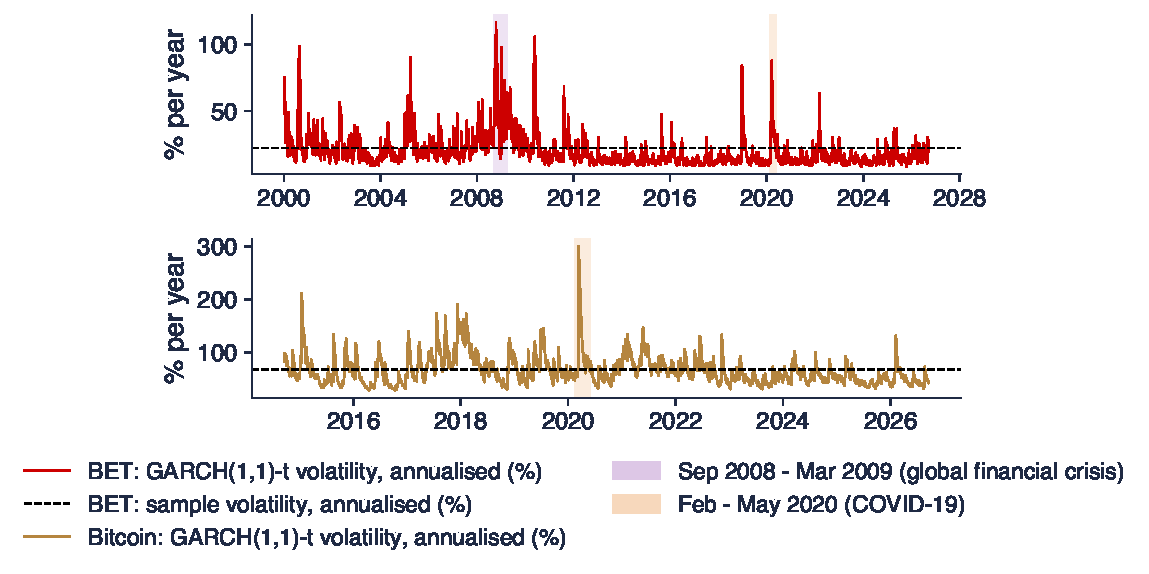
\includegraphics[width=0.97\textwidth,height=0.56\textheight,keepaspectratio]{sfm_ch9_vol_bet_btc.pdf}
\end{center}
\vspace{-0.25cm}
\begin{itemize}
    \item BET: cel mai înalt vîrf în 2008 (117\%, 15 octombrie 2008), mai mic în 2020 (88\%); Bitcoin: 301\% pe 13 martie 2020, mediana 59\%
    \item Interpretare: șocul din 2020 a afectat toate piețele în aceeași săptămînă; volatilitatea mediană a Bitcoin este de 4{,}1 ori mai mare decît cea a S\&P 500 (14\%)
\end{itemize}
\sfmquantlet{Ch_09}{SFM_ch9_volatility_markets}
\end{frame}

\begin{frame}{Durata unui șoc de volatilitate}
\itemsize{\footnotesize}
\begin{center}
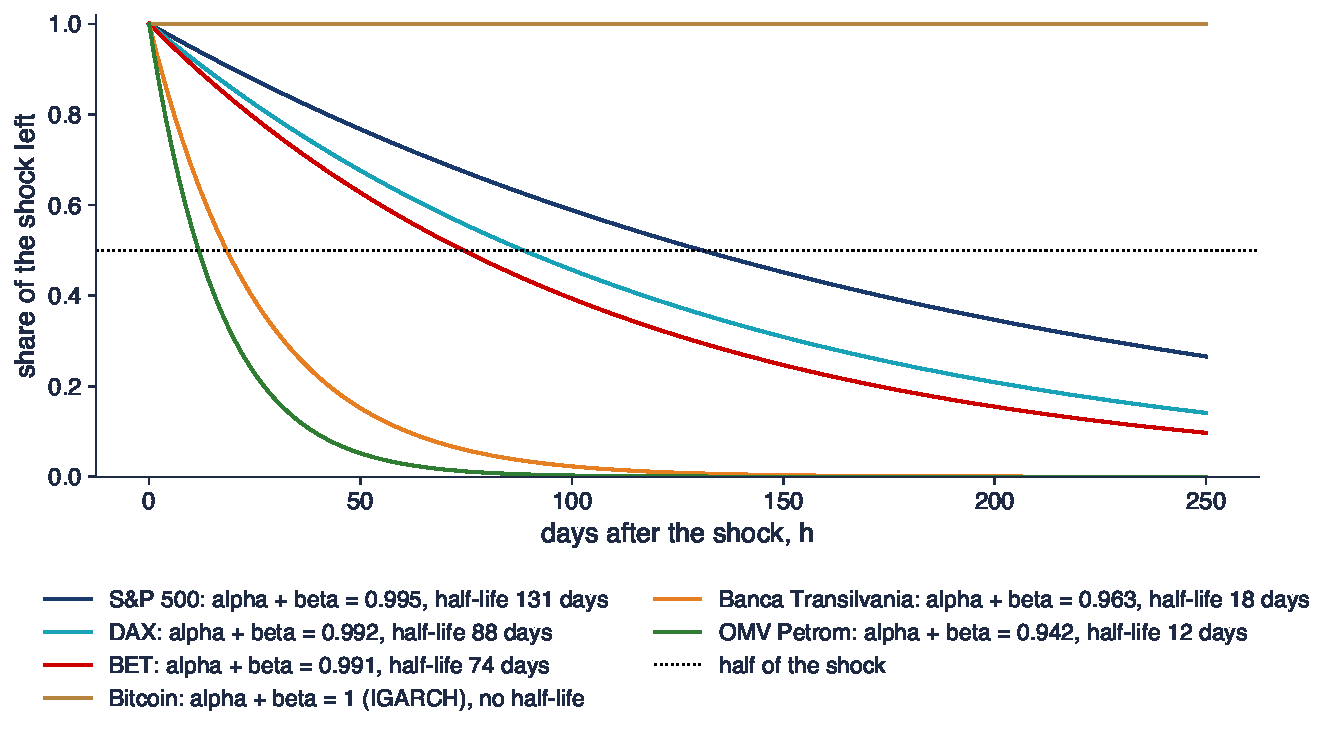
\includegraphics[width=0.97\textwidth,height=0.52\textheight,keepaspectratio]{sfm_ch9_persistence.pdf}
\end{center}
\vspace{-0.25cm}
\begin{itemize}
    \item Ponderea unui șoc de varianță rămasă după $h$ zile: $(\alpha + \beta)^h$; timpul de înjumătățire este punctul în care curba trece de 1/2
    \item Interpretare: după o criză, S\&P 500 are nevoie de circa jumătate de an ca să înjumătățească varianța în exces; OMV Petrom de circa două săptămîni; Bitcoin, niciodată
\end{itemize}
\sfmquantlet{Ch_09}{SFM_ch9_volatility_markets}
\end{frame}


%=============================================================================
\section{Asimetria și efectul de levier}
%=============================================================================

\begin{frame}{Efectul de levier}
\itemsize{\small}
\begin{itemize}
    \item Efectul de levier din secțiunea 1 \refChristie{} are două explicații
    \begin{itemize}
        \item explicația prin \textbf{levier}: un preț mai mic al acțiunii crește raportul datorii/capitaluri proprii, deci acțiunea devine mai riscantă
        \item \textbf{feedback-ul volatilității}: știrile despre un risc mai mare scad imediat prețurile
    \end{itemize}
    \item GARCH(1,1) nu îl poate surprinde: $\sigma_t^2$ depinde de $\varepsilon_{t-1}^2$, nu de semnul lui $\varepsilon_{t-1}$
    \begin{itemize}
        \item graficul QQ din secțiunea 6 și t asimetrică ($\hat\lambda < 0$) au arătat deja spre coada stîngă
    \end{itemize}
    \item \textbf{NIC} (news impact curve, curba de impact a știrilor) \refEN: $\sigma_t^2$ ca funcție de $\varepsilon_{t-1}$, cu $\sigma_{t-1}^2$ fixat la varianța necondiționată
\end{itemize}
\end{frame}

\begin{frame}{GJR-GARCH și EGARCH}
\itemsize{\small}
\begin{itemize}
    \item \textbf{GJR-GARCH} \refGJR: $\sigma_t^2 = \omega + (\alpha + \gamma\,I_{t-1})\,\varepsilon_{t-1}^2 + \beta\sigma_{t-1}^2$, $I_{t-1} = 1$ dacă $\varepsilon_{t-1} < 0$, altfel 0
    \begin{itemize}
        \item $I_{t-1}$: un indicator al unui șoc negativ ieri; $\gamma$: reacția suplimentară la știrile proaste
        \item știri bune: panta $\alpha$; știri proaste: $\alpha + \gamma$; efect de levier: $\gamma > 0$
        \item persistența $\alpha + \beta + \gamma/2$ pentru $z_t$ simetric (jumătate dintre șocuri sînt negative)
    \end{itemize}
    \item \textbf{EGARCH} (exponential GARCH, GARCH exponențial) \refNelson: $\ln\sigma_t^2 = \omega + \alpha\big(|z_{t-1}| - E|z_{t-1}|\big) + \gamma z_{t-1} + \beta\ln\sigma_{t-1}^2$
    \begin{itemize}
        \item $|z_{t-1}| - E|z_{t-1}|$: mărimea șocului standardizat de ieri peste media ei ($E|z| = \sqrt{2/\pi}$ pentru $z$ Normal)
        \item logaritmul păstrează $\sigma_t^2 > 0$ fără restricții de semn asupra parametrilor
        \item efect de levier: $\gamma < 0$ (un $z_{t-1}$ negativ crește $\ln\sigma_t^2$); persistența: $\beta$
    \end{itemize}
    \item Ambele modele, precum și GARCH cu prag (threshold GARCH), sînt tratate în \refFHH, secțiunea 13.2
\end{itemize}
\end{frame}

\begin{frame}{Curbele de impact ale știrilor: S\&P 500 și Bitcoin}
\itemsize{\footnotesize}
\begin{center}
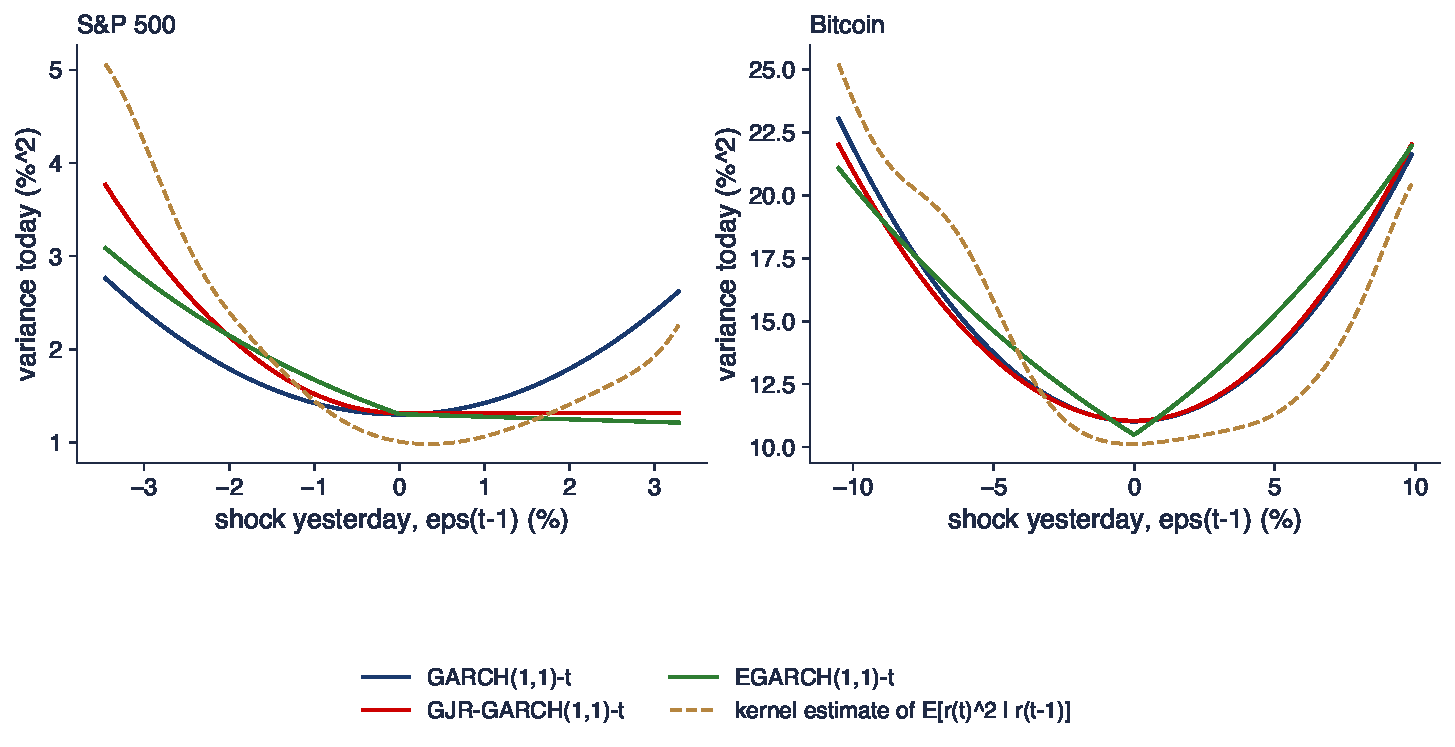
\includegraphics[width=0.97\textwidth,height=0.50\textheight,keepaspectratio]{sfm_ch9_nic.pdf}
\end{center}
\vspace{-0.25cm}
\begin{itemize}
    \item Curbele modelelor: $\sigma_t^2$ în funcție de $\varepsilon_{t-1}$, cu $\sigma_{t-1}^2$ fixat la varianța de selecție; linia întreruptă: o estimare nucleu (Nadaraya--Watson) a lui $E[r_t^2 \mid r_{t-1}]$, ideea din SFENewsImpactCurve
    \item S\&P 500, GJR: după o scădere de 2\%, varianța de mîine este de 1{,}62 ori mai mare decît după o creștere de 2\%; Bitcoin: raportul 1{,}00, o curbă simetrică
\end{itemize}
\sfmquantlet{Ch_09}{SFM_ch9_asymmetry}
\end{frame}

\begin{frame}{Asimetria pe șase piețe}
\itemsize{\footnotesize}
\begin{center}
\scriptsize
\begin{tabular}{lrrrrrrr}
\toprule
& GJR $\alpha$ & GJR $\gamma$ & $t(\gamma)$ & LR & p & EGARCH $\gamma$ & $t(\gamma)$ \\
\midrule
S\&P 500 & $0{,}000$ & $0{,}205$ & $10{,}0$ & $235{,}7$ & $<$\,0{,}001 & ${-0{,}165}$ & ${-15{,}2}$ \\
DAX & $0{,}000$ & $0{,}163$ & $8{,}7$ & $204{,}5$ & $<$\,0{,}001 & ${-0{,}133}$ & ${-11{,}8}$ \\
BET & $0{,}172$ & $0{,}043$ & $2{,}1$ & $4{,}9$ & 0{,}026 & ${-0{,}028}$ & ${-2{,}6}$ \\
Bitcoin & $0{,}113$ & $-0{,}013$ & $-0{,}7$ & $0{,}7$ & 0{,}416 & ${0{,}015}$ & ${1{,}2}$ \\
TLV & $0{,}101$ & $0{,}065$ & $2{,}7$ & $7{,}8$ & 0{,}005 & ${-0{,}040}$ & ${-3{,}0}$ \\
SNP & $0{,}117$ & $0{,}033$ & $1{,}4$ & $1{,}7$ & 0{,}188 & ${-0{,}027}$ & ${-1{,}9}$ \\
\bottomrule
\end{tabular}
\end{center}
\begin{itemize}
    \item Inovații Student-t; statistici $t$ cu SE robuste; LR (likelihood ratio, raportul de verosimilitate) $= 2(\ell_{GJR} - \ell_{GARCH}) \sim \chi^2(1)$
    \item S\&P 500 și DAX: GJR $\hat\alpha = 0$: doar știrile proaste cresc volatilitatea; un efect de levier foarte puternic
    \item BET și TLV: un efect slab, semnificativ după testul LR, dar BIC preferă modelul GARCH simetric; SNP: nesemnificativ la 5\%; Bitcoin: niciun efect (în EGARCH, $\gamma$ este ușor pozitiv și nesemnificativ)
    \item Interpretare: efectul de levier este o proprietate a piețelor mature de acțiuni; la cripto, creșterile mari cresc volatilitatea la fel de mult ca scăderile mari
\end{itemize}\sfmquantlet{Ch_09}{SFM_ch9_asymmetry}
\end{frame}


%=============================================================================
\section{Diagnostic}
%=============================================================================

\begin{frame}{Verificarea unui model estimat}
\itemsize{\small}
\begin{itemize}
    \item Dacă modelul este corect, \textbf{reziduurile standardizate} $\hat z_t = (r_t - \hat\mu)/\hat\sigma_t$ sînt aproape i.i.d., cu media 0 și varianța 1
    \begin{itemize}
        \item \textbf{LB} (Ljung--Box) $Q(10)$ pe $\hat z_t$: nu a rămas autocorelație în medie (\sfmchlink{https://danpele.github.io/SFM/RO/Cursuri/capitol7_piete_eficiente_mers_aleator_vr.pdf}{Capitolul 7}) \refLjung
        \item $Q(10)$ pe $\hat z_t^2$ și testul ARCH-LM: nu au rămas efecte ARCH (\sfmchlink{https://danpele.github.io/SFM/RO/Cursuri/capitol8_estimatori_volatilitate.pdf}{Capitolul 8})
        \item graficul QQ al lui $\hat z_t$: este corectă distribuția presupusă? (secțiunea 6)
    \end{itemize}
    \item \textbf{Testul de asimetrie (sign bias)} \refEN: regresia lui $\hat z_t^2$ pe $I_{t-1}$, $I_{t-1}\hat\varepsilon_{t-1}$ și $(1 - I_{t-1})\hat\varepsilon_{t-1}$
    \begin{itemize}
        \item testul comun $T R^2 \sim \chi^2(3)$: o respingere înseamnă că semnul șocurilor trecute încă anticipează varianța (lipsește asimetria)
    \end{itemize}
    \item Un diagnostic fără respingere nu dovedește că modelul este corect; o respingere arată unde greșește
\end{itemize}
\end{frame}

\begin{frame}{Autocorelațiile eliminate de GARCH}
\itemsize{\footnotesize}
\begin{center}
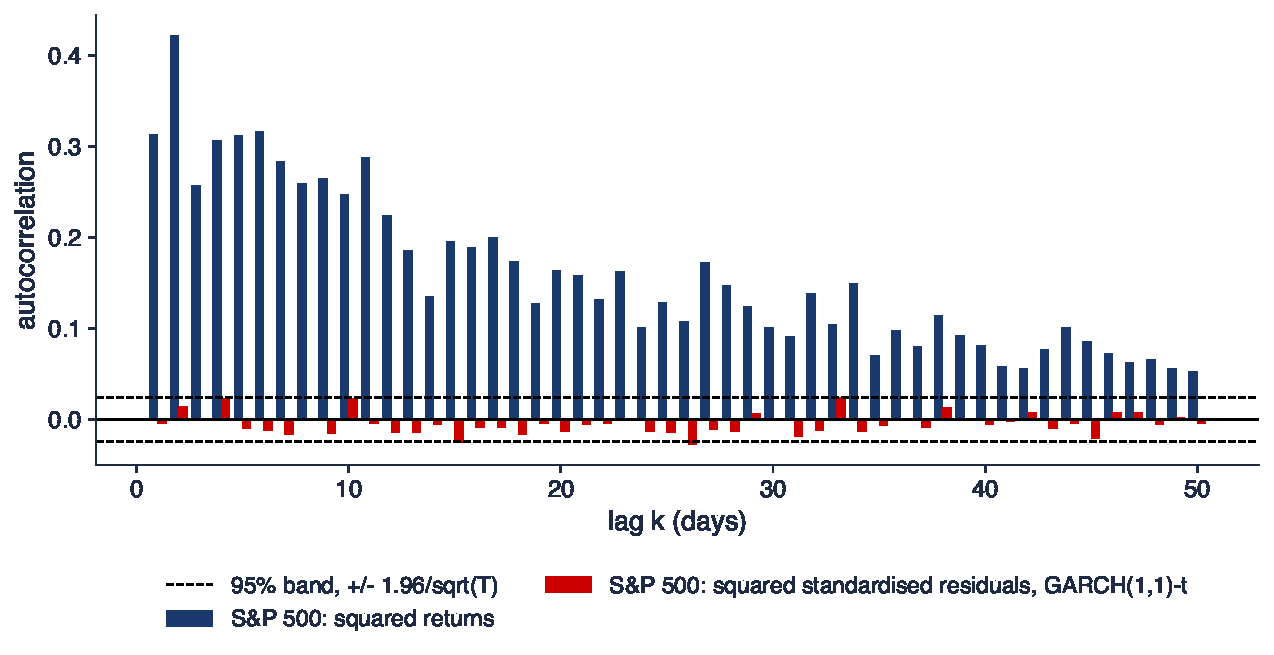
\includegraphics[width=0.97\textwidth,height=0.50\textheight,keepaspectratio]{sfm_ch9_acf_diag.pdf}
\end{center}
\vspace{-0.25cm}
\begin{itemize}
    \item ACF a lui $r_t^2$: $0{,}31$ la lagul 1 și încă $0{,}053$ la lagul 50; ACF a lui $\hat z_t^2$ (GARCH(1,1)-t): $-0{,}005$ la lagul 1, cel mult $0{,}028$ în valoare absolută; banda $\pm0{,}024$
    \item Interpretare: trei parametri absorb aproape tot volatility clustering din datele zilnice de după 2000
\end{itemize}
\sfmquantlet{Ch_09}{SFM_ch9_diagnostics}
\end{frame}

\begin{frame}{Diagnostic pe date reale}
\itemsize{\footnotesize}
\begin{center}
\scriptsize
\begin{tabular}{lrrrr}
\toprule
S\&P 500 & $Q(10)$ (p) & $Q(10)$ al pătratelor (p) & ARCH-LM(5) (p) & sign bias $\chi^2(3)$ (p) \\
\midrule
randamente $r_t$ & $96{,}3$ ($<$\,0{,}001) & $6133$ ($<$\,0{,}001) & $1679$ ($<$\,0{,}001) & -- \\
$\hat z_t$, GARCH Normal & $21{,}2$ (0{,}020) & $16{,}4$ (0{,}089) & $8{,}0$ (0{,}154) & -- \\
$\hat z_t$, GARCH-t & $21{,}9$ (0{,}016) & $13{,}6$ (0{,}192) & $5{,}8$ (0{,}326) & $40{,}7$ ($<$\,0{,}001) \\
\bottomrule
\end{tabular}
\end{center}
\begin{itemize}
    \item GARCH elimină efectele ARCH ($Q(10)$ al pătratelor: de la $6133$ la $13{,}6$); rămîne puțină autocorelație în medie (modelul are media constantă)
    \item Testul de asimetrie respinge pentru GARCH simetric ($t$ al semnului $= 3{,}56$): lipsește asimetria din secțiunea 8; la fel pentru DAX (p $<$\,0{,}001) și BET (p = 0{,}009)
    \item Celelalte piețe, $Q(10)$ al lui $\hat z_t^2$ (GARCH-t): p între 0{,}115 (DAX) și 0{,}993 (TLV): nu a rămas niciun efect ARCH
\end{itemize}\sfmquantlet{Ch_09}{SFM_ch9_diagnostics}
\end{frame}


%=============================================================================
\section{Alegerea modelului}
%=============================================================================

\begin{frame}{Nouă modele pentru S\&P 500}
\itemsize{\footnotesize}
\begin{itemize}
    \item \textbf{AIC} (Akaike information criterion, criteriul informațional Akaike) $= -2\ell + 2k$ \refAkaike; \textbf{BIC} (Bayesian information criterion, criteriul informațional bayesian) $= -2\ell + k\ln T$ \refSchwarz; $\ell$: log-verosimilitatea maximă, $k$ parametri, $T$ observații; valoarea mai mică este mai bună (\sfmchlink{https://danpele.github.io/SFM/RO/Cursuri/capitol6_selectia_modelului_managementul_riscului.pdf}{Capitolul 6})
\end{itemize}\begin{center}
\scriptsize
\begin{tabular}{lrrrrrr}
\toprule
& \multicolumn{2}{c}{Normal} & \multicolumn{2}{c}{Student-t} & \multicolumn{2}{c}{t asimetrică} \\ & log-verosim. & $\Delta$BIC & log-verosim. & $\Delta$BIC & log-verosim. & $\Delta$BIC \\
\midrule
GARCH(1,1) & \ensuremath{-}9218{,}0 & 648{,}9 & \ensuremath{-}9062{,}5 & 346{,}7 & \ensuremath{-}9038{,}4 & 307{,}4 \\
GJR-GARCH(1,1) & \ensuremath{-}9086{,}5 & 394{,}7 & \ensuremath{-}8944{,}6 & 119{,}9 & \ensuremath{-}8905{,}1 & 49{,}6 \\
EGARCH(1,1) & \ensuremath{-}9075{,}6 & 372{,}9 & \ensuremath{-}8922{,}1 & 74{,}8 & \ensuremath{-}8880{,}3 & 0{,}0 \\
\bottomrule
\end{tabular}
\end{center}
\begin{itemize}
    \item $\Delta$BIC: diferența față de cel mai bun model; AIC dă aceeași ordine
    \item Ambele alegeri contează: pornind de la GARCH cu inovații Normale, doar asimetria (EGARCH cu inovații Normale) reduce BIC cu 276, doar cozile groase (GARCH cu t asimetrică) cu 341, iar ambele împreună cu 649
    \item Interpretare: EGARCH cu inovații t asimetrice cîștigă; cu 6\,714 observații chiar și îmbunătățirile mici sînt „semnificative”; comparația prognozelor din secțiunea 11 este testul real
\end{itemize}\sfmquantlet{Ch_09}{SFM_ch9_diagnostics}
\end{frame}


%=============================================================================
\section{Prognoza volatilității}
%=============================================================================

\begin{frame}{Prognoze pe mai mulți pași}
\itemsize{\small}
\begin{itemize}
    \item Un pas: $\sigma_{t+1}^2 = \omega + \alpha\varepsilon_t^2 + \beta\sigma_t^2$ este cunoscut la sfîrșitul zilei $t$
    \begin{itemize}
        \item doi pași: $E_t[\sigma_{t+2}^2] = \omega + \alpha E_t[\varepsilon_{t+1}^2] + \beta\sigma_{t+1}^2 = \omega + (\alpha + \beta)\sigma_{t+1}^2$, deoarece $E_t[\varepsilon_{t+1}^2] = \sigma_{t+1}^2$
    \end{itemize}
    \item Prin inducție: $E_t[\sigma_{t+h}^2] = \bar\sigma^2 + (\alpha + \beta)^{h-1}(\sigma_{t+1}^2 - \bar\sigma^2)$
    \begin{itemize}
        \item $E_t$: media condiționată de informația de la sfîrșitul zilei $t$; $h$: orizontul, în zile
        \item prognoza converge spre varianța pe termen lung; viteza este dată de $\alpha + \beta$
    \end{itemize}
    \item Varianța randamentului pe $H$ zile: suma prognozelor zilnice (randamentele sînt necorelate)
    \begin{itemize}
        \item $\mathrm{Var}_t(r_{t+1} + \dots + r_{t+H}) = \sum_{h=1}^{H} E_t[\sigma_{t+h}^2]$, nu $H\sigma_{t+1}^2$
        \item regula rădăcinii pătrate a timpului, $\sigma_{t+1}\sqrt{H}$, dă valori prea mari în criză și prea mici într-o perioadă liniștită
    \end{itemize}
\end{itemize}
\end{frame}

\begin{frame}{Exemplu rezolvat: S\&P 500 la 18 septembrie 2026}
\itemsize{\small}
\begin{itemize}
    \item GARCH(1,1)-t: $\alpha + \beta = 0{,}9947$, $\bar\sigma^2 = 2{,}972$; prognoza pentru ziua următoare $\sigma_{t+1}^2 = 0{,}509$ (sub nivelul pe termen lung)
    \item Pas cu pas
    \begin{itemize}
        \item ziua 10: $2{,}972 + 0{,}9947^{9}(0{,}509 - 2{,}972) = 2{,}972 + 0{,}953 \times (0{,}509 - 2{,}972) = 0{,}624$
        \item varianța pe 10 zile: suma celor zece prognoze zilnice $= 5{,}67$, deci volatilitatea pe 10 zile este $2{,}38\%$
        \item regula rădăcinii pătrate a timpului: $\sqrt{10 \times 0{,}509} = 2{,}26\%$: prea mică, deoarece volatilitatea este așteptată să crească spre nivelul ei pe termen lung
    \end{itemize}
\end{itemize}
\end{frame}

\begin{frame}{Structura la termen a volatilității}
\itemsize{\footnotesize}
\begin{center}
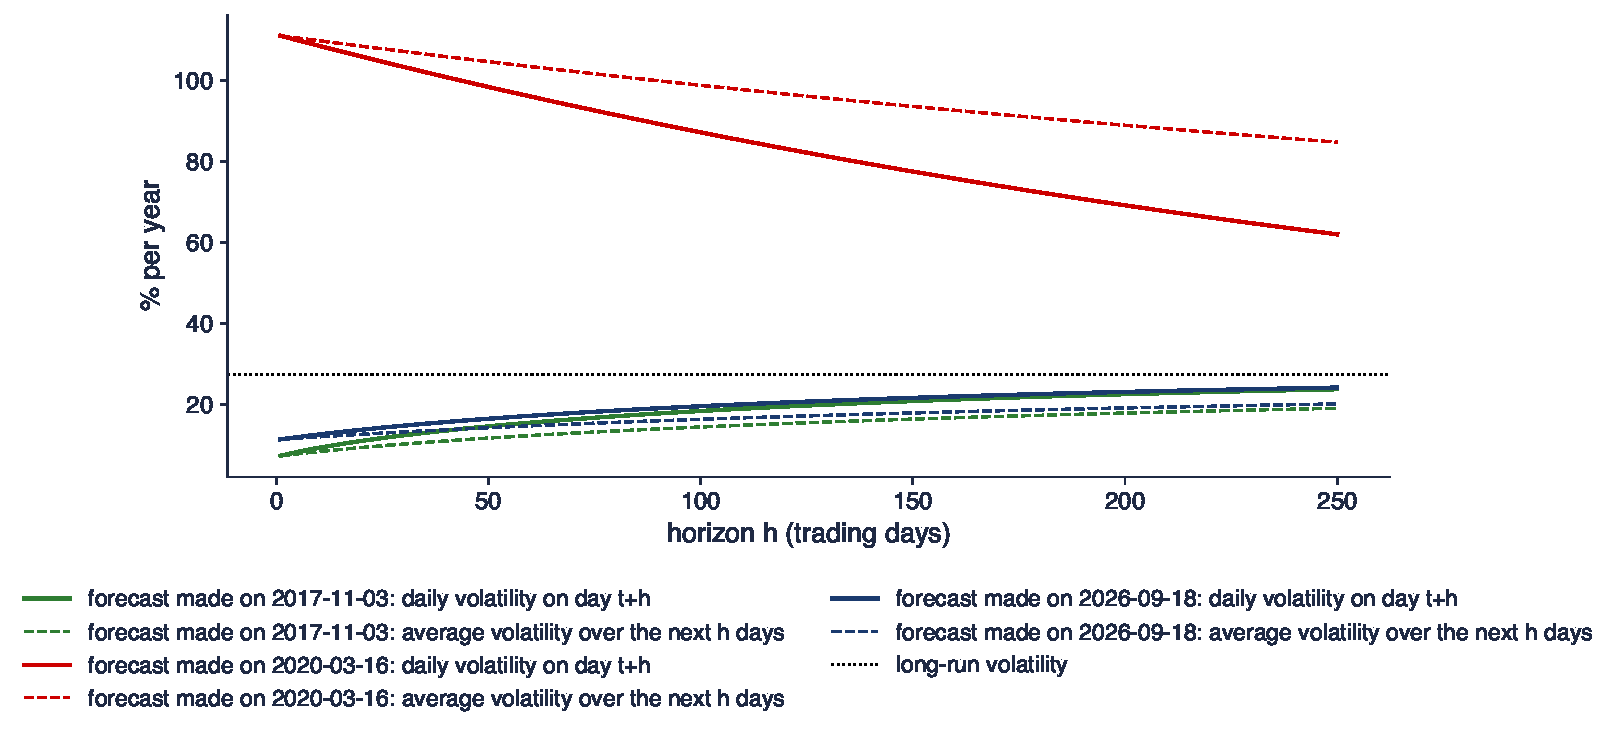
\includegraphics[width=0.97\textwidth,height=0.50\textheight,keepaspectratio]{sfm_ch9_term_structure.pdf}
\end{center}
\vspace{-0.25cm}
\begin{itemize}
    \item S\&P 500, GARCH(1,1)-t estimat pe toate datele; prognoze făcute într-o zi liniștită (3 noiembrie 2017), în vîrful pandemiei COVID-19 (16 martie 2020) și la 18 septembrie 2026
    \item Ziua liniștită: 7{,}3\% mîine, în medie 19{,}0\% pe un an; vîrful COVID-19: 111{,}0\% mîine, încă 84{,}7\% în medie pe un an
    \item Interpretare: toate curbele se îndreaptă spre nivelul pe termen lung (27{,}3\%) cu aceeași viteză redusă: panta structurii la termen arată dacă sîntem într-o perioadă liniștită sau într-una turbulentă
\end{itemize}
\sfmquantlet{Ch_09}{SFM_ch9_forecasts}
\end{frame}

\begin{frame}{Evaluarea unei prognoze de volatilitate}
\itemsize{\small}
\begin{itemize}
    \item Adevăratul $\sigma_t^2$ nu este observat niciodată: comparăm prognoza $h_t$ cu o \textbf{aproximare} zgomotoasă, aici $r_t^2$
    \begin{itemize}
        \item $E_{t-1}[r_t^2] = \sigma_t^2$ (cu $\mu \approx 0$), dar $r_t^2$ este foarte zgomotos: un $R^2$ mic chiar și pentru o prognoză perfectă \refAB
    \end{itemize}
    \item Funcția de pierdere \textbf{QLIKE} \refPatton: $L(r_t^2, h_t) = \dfrac{r_t^2}{h_t} + \ln h_t$ (pînă la o constantă); valoarea mai mică este mai bună
    \begin{itemize}
        \item $h_t$: prognoza varianței pentru ziua $t$, făcută la sfîrșitul zilei $t-1$
        \item ordonează corect prognozele chiar și cu o aproximare zgomotoasă; este minus log-verosimilitatea Normală
        \item penalizează mai mult prognozele prea mici decît pe cele prea mari
    \end{itemize}
    \item \textbf{În afara eșantionului}: din 2015, fiecare prognoză folosește doar date pînă în ziua precedentă; modelele se reestimează la fiecare 250 de zile
    \begin{itemize}
        \item testul \textbf{DM} (Diebold--Mariano) \refDM: este diferența medie a pierderilor egală cu zero? $t$ cu erori standard HAC (heteroskedasticity and autocorrelation consistent, robuste la heteroscedasticitate și autocorelație)
    \end{itemize}
\end{itemize}
\end{frame}

\begin{frame}{GARCH față de EWMA, în afara eșantionului}
\itemsize{\scriptsize}
\begin{center}
\scriptsize
\begin{tabular}{lrrrrr}
\toprule
2015--2026 & zile & QLIKE GARCH-t & QLIKE GJR-t & QLIKE EWMA & DM $t$, GARCH-t față de EWMA (p) \\
\midrule
S\&P 500 & 2\,944 & $0{,}761$ & $0{,}733$ & $0{,}819$ & ${-3{,}69}$ ($<$\,0{,}001) \\
DAX & 2\,973 & $1{,}090$ & $1{,}064$ & $1{,}121$ & ${-3{,}19}$ (0{,}001) \\
BET & 2\,926 & $0{,}680$ & $0{,}674$ & $0{,}788$ & ${-2{,}22}$ (0{,}027) \\
Bitcoin & 4\,279 & $3{,}383$ & $3{,}401$ & $3{,}390$ & ${-0{,}20}$ (0{,}845) \\
\bottomrule
\end{tabular}
\end{center}
\vspace{-1mm}
\begin{center}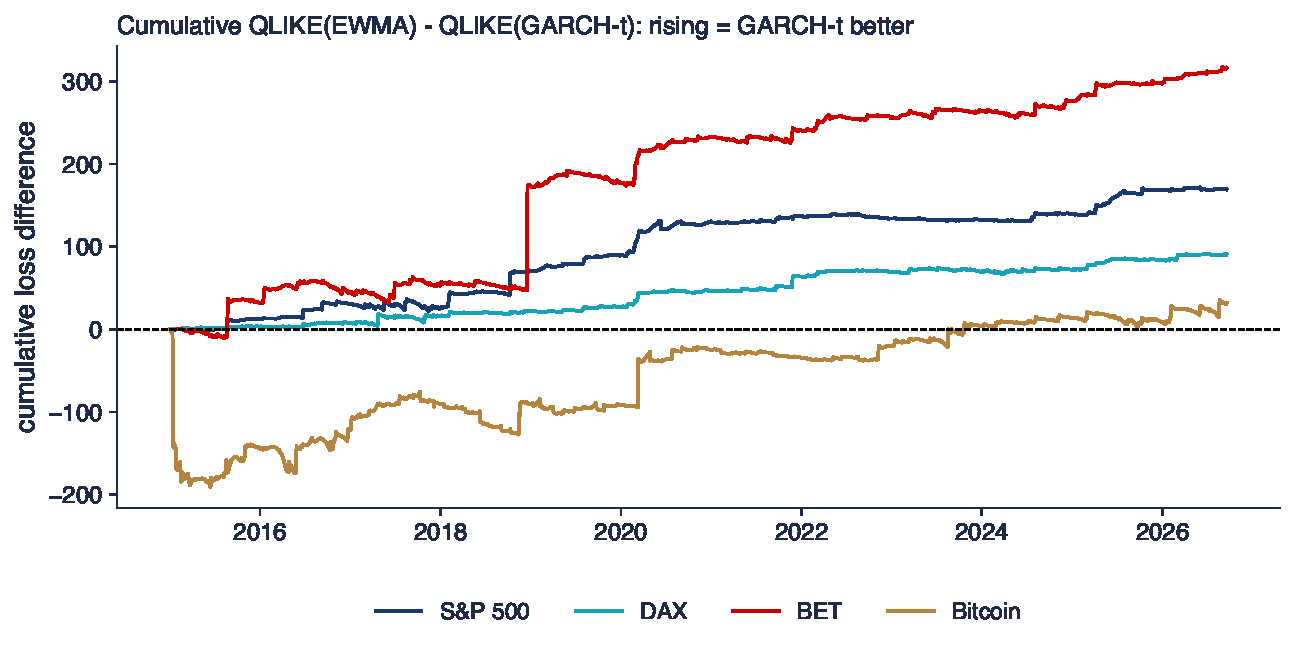
\includegraphics[width=0.80\textwidth,height=0.34\textheight,keepaspectratio]{sfm_ch9_forecast_eval.pdf}\end{center}
\vspace{-3mm}
\begin{itemize}
    \item Indicii de acțiuni: GARCH-t este mai bun decît EWMA ($t < -2$); GJR-t este și mai bun pentru S\&P 500, DAX și BET
    \item Interpretare: Bitcoin: nicio diferență ($t = -0{,}20$): GARCH-ul lui este un IGARCH, adică aproape un EWMA (secțiunea 7)
\end{itemize}\sfmquantlet{Ch_09}{SFM_ch9_forecasts}
\end{frame}


%=============================================================================
\section{VaR 1\% dintr-un model GARCH}
%=============================================================================

\begin{frame}{VaR condiționat}
\itemsize{\small}
\begin{itemize}
    \item \textbf{VaR} la nivelul $\alpha$ (value at risk, valoarea expusă la risc): pierderea depășită cu probabilitatea $\alpha$: $\mathrm{VaR}_\alpha = -q_\alpha(r_{t+1})$ (\sfmchlink{https://danpele.github.io/SFM/RO/Cursuri/capitol6_selectia_modelului_managementul_riscului.pdf}{Capitolul 6})
    \begin{itemize}
        \item aici $\alpha$ este nivelul VaR, nu parametrul GARCH; $q_\alpha$: cuantila de ordin $\alpha$
        \item aici $\alpha = 1\%$: VaR 1\%, o pierdere depășită într-o zi din o sută
    \end{itemize}
    \item Cu $r_{t+1} = \mu + \sigma_{t+1}z_{t+1}$: $\mathrm{VaR}_{t+1} = -(\mu + \sigma_{t+1}\,q_\alpha(z))$
    \begin{itemize}
        \item Normală: $q_{0{,}01} = -2{,}326$; t standardizată: $q_{0{,}01} = t_\nu^{-1}(0{,}01)\sqrt{(\nu - 2)/\nu}$
        \item $t_\nu^{-1}(0{,}01)$: cuantila de 1\% a distribuției Student-t cu $\nu$ grade de libertate; rădăcina o rescalează la varianța 1
        \item VaR se schimbă în fiecare zi odată cu $\sigma_{t+1}$: mare în perioadele turbulente, mic în perioadele liniștite
    \end{itemize}
    \item \textbf{Exemplu rezolvat}: S\&P 500 la 18 septembrie 2026, GARCH(1,1)-t: $\hat\mu = 0{,}079$, $\sigma_{t+1} = 0{,}714$, $\hat\nu = 6{,}26$
    \begin{itemize}
        \item $q_{0{,}01}(z) = -3{,}100 \times 0{,}825 = -2{,}557$; VaR 1\% $= -(0{,}079 + 0{,}714 \times (-2{,}557)) = 1{,}75\%$
        \item cu $z_t$ Normale: $1{,}58\%$; pe 10 zile (suma varianțelor, fără $\mu$): $2{,}557 \times \sqrt{5{,}67}$, circa $6{,}09\%$
    \end{itemize}
\end{itemize}
\end{frame}

\begin{frame}{VaR 1\% în timpul crahului COVID-19}
\itemsize{\footnotesize}
\begin{center}
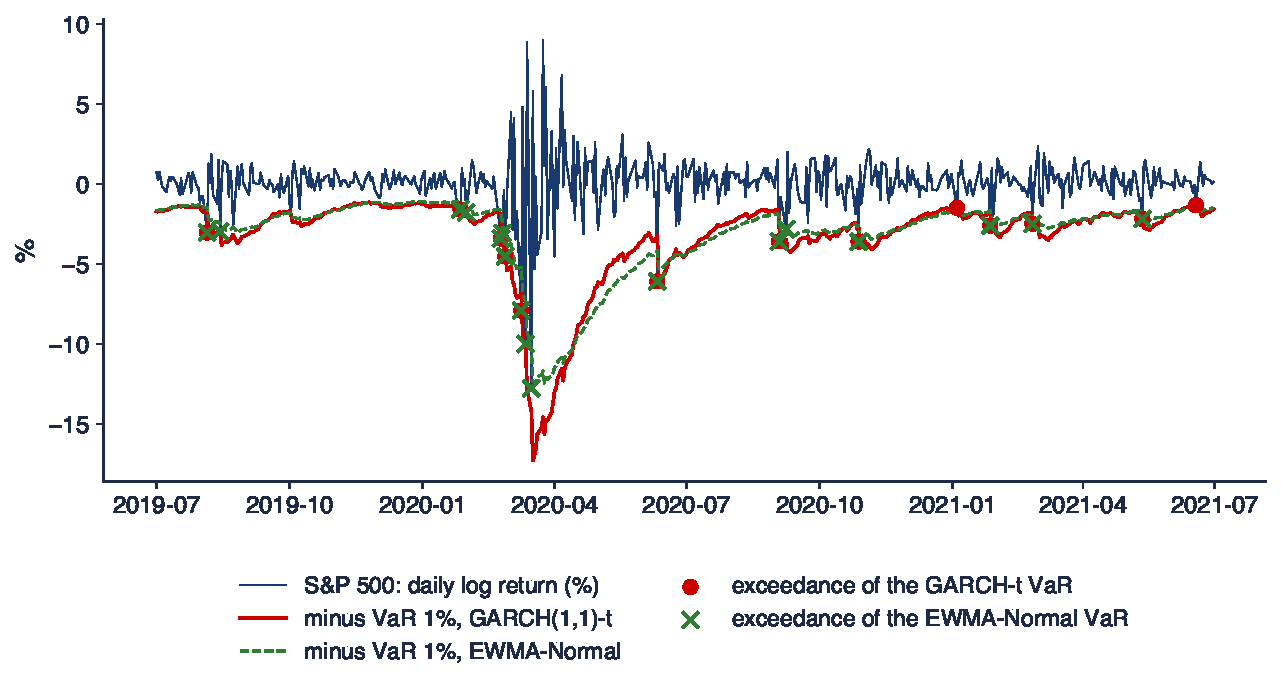
\includegraphics[width=0.97\textwidth,height=0.50\textheight,keepaspectratio]{sfm_ch9_var.pdf}
\end{center}
\vspace{-0.25cm}
\begin{itemize}
    \item S\&P 500, iulie 2019 -- iunie 2021 (505 zile): VaR 1\% pe o zi din GARCH(1,1)-t (reestimat la fiecare 250 de zile) și din EWMA cu $z_t$ Normale
    \item Depășiri (randament sub $-$VaR): GARCH-t 13, EWMA-Normal 17; așteptat circa 5; ambele modele reacționează, dar abia după primele scăderi mari din martie 2020
\end{itemize}
\sfmquantlet{Ch_09}{SFM_ch9_forecasts}
\end{frame}

\begin{frame}{Depășiri 2015--2026: o primă privire asupra backtesting-ului}
\itemsize{\footnotesize}
\begin{center}
\footnotesize
\begin{tabular}{lrrrr}
\toprule
VaR 1\% & zile & așteptat & GARCH-t & EWMA-Normal \\
\midrule
S\&P 500 & 2\,944 & 29 & 49 (1{,}66\%) & 65 (2{,}21\%) \\
DAX & 2\,973 & 30 & 45 (1{,}51\%) & 74 (2{,}49\%) \\
BET & 2\,926 & 29 & 34 (1{,}16\%) & 67 (2{,}29\%) \\
Bitcoin & 4\,279 & 43 & 64 (1{,}50\%) & 93 (2{,}17\%) \\
\bottomrule
\end{tabular}
\end{center}
\begin{itemize}
    \item Un VaR 1\% corect este depășit în 1\% dintre zile, iar depășirile nu apar grupat
    \item EWMA-Normal: 2{,}2--2{,}5\%: cuantila Normală este prea mică pentru cozi groase
    \item GARCH-t: 1{,}2--1{,}7\%: mult mai aproape de 1\%, dar tot peste 1\% pentru S\&P 500 și DAX (lipsește efectul de levier)
    \item Sînt aceste diferențe semnificative? \sfmchlink{https://danpele.github.io/SFM/RO/Cursuri/capitol10_var_es_backtesting.pdf}{Capitolul 10}: testul \refKupiec, ES 2,5\%, backtesting
    \item Lectură suplimentară despre prognoza VaR pentru Bitcoin: \refPeleB
\end{itemize}\sfmquantlet{Ch_09}{SFM_ch9_forecasts}
\end{frame}


%=============================================================================
\section{AI pentru descoperire științifică}
%=============================================================================

\begin{frame}{O întrebare deschisă}
\itemsize{\small}
\begin{itemize}
    \item \textbf{Devine volatilitatea Bitcoin mai asemănătoare cu volatilitatea unui indice de acțiuni?}
    \begin{itemize}
        \item azi: IGARCH, $\hat\nu = 3{,}18$, fără efect de levier; S\&P 500: revenire la medie, efect de levier puternic
        \item din 2024, ETF-urile (exchange-traded funds, fonduri tranzacționate la bursă) pe Bitcoin aduc investitorii din piața de acțiuni pe piața cripto
    \end{itemize}
    \item Dovezi anterioare despre activele cripto ca o clasă de active: \refPeleC; volatilitatea ca informație: \refPeleA
    \item Întrebarea rămîne deschisă: schimbările de regim, prăbușirea pieței cripto din 2022 și lansarea ETF-urilor se suprapun; răspunsul depinde de fereastra aleasă
    \item Instrumentele AI pot accelera un astfel de studiu, dar rezultatele lui trebuie verificate \refWang
\end{itemize}
\end{frame}

\begin{frame}{Contribuția posibilă a AI}
\itemsize{\small}
\begin{itemize}
    \item \textbf{Literatura}: o listă a studiilor despre modelele GARCH pentru active cripto și a modelelor folosite
    \item \textbf{Cod}: o primă versiune a estimărilor GJR-GARCH-t pe ferestre mobile pentru Bitcoin și S\&P 500, cu pachetul \texttt{arch}
    \item \textbf{Robustețe}: alte ferestre, Ethereum, eliminarea zilelor de weekend, inovații t asimetrice
    \item Exemplu de prompt
    \begin{itemize}
        \item \aiprompt{Write Python code that estimates a GJR-GARCH(1,1) model with Student-t innovations on daily Bitcoin and S\&P 500 log returns in percent, on rolling windows of 750 days moved by 21 days, and plots the persistence, gamma and nu over time.}
    \end{itemize}
\end{itemize}
\end{frame}

\begin{frame}{Verificări necesare}
\itemsize{\small}
\begin{itemize}
    \item Unitățile: randamente în \% (nu în zecimale), altfel algoritmul de optimizare se poate opri la un $\omega$ greșit
    \item Persistența GJR este $\alpha + \beta + \gamma/2$, nu $\alpha + \beta$; pentru EGARCH este $\beta$
    \item Estimările pe frontieră ($\alpha + \beta = 1$): fără timp de înjumătățire și fără volatilitate pe termen lung; nu raportăm valori infinite
    \item Calendarele: Bitcoin se tranzacționează 7 zile pe săptămînă, S\&P 500 cinci; anualizăm fiecare serie cu propria frecvență
    \item Ferestrele mobile se suprapun: estimările consecutive nu sînt dovezi independente
    \item Referințele: fiecare lucrare citată trebuie să existe; verificați DOI-ul
\end{itemize}
\end{frame}

\begin{frame}{Idee de proiect}
\itemsize{\small}
\begin{itemize}
    \item \textbf{Întrebarea}: s-a apropiat volatilitatea Bitcoin de volatilitatea acțiunilor după 2021?
    \begin{itemize}
        \item date: Bitcoin din 2014, Ethereum din 2015, S\&P 500 și BET (EODHD)
    \end{itemize}
    \item Pași
    \begin{itemize}
        \item GJR-GARCH-t pe 2015--2019 și pe 2021--2026: persistența, $\gamma$, $\nu$
        \item corelația volatilităților GARCH ale Bitcoin și S\&P 500 în fiecare perioadă
        \item QLIKE în afara eșantionului pentru GARCH față de EWMA, în fiecare perioadă
    \end{itemize}
    \item Livrabil: un tabel, un grafic și un paragraf despre ce pot și ce nu pot arăta datele
    \item Declarați orice utilizare a instrumentelor AI și enumerați erorile acestora pe care le-ați corectat
\end{itemize}
\end{frame}


%=============================================================================
\section{Rezumat}
%=============================================================================

\begin{frame}{Idei de reținut}
\itemsize{\small}
\begin{itemize}
    \item Randamentele: media imprevizibilă, varianța previzibilă: $r_t = \mu + \sigma_t z_t$
    \item GARCH(1,1), cu trei parametri, surprinde volatility clustering în toate seriile noastre; $\alpha + \beta$ este apropiat de 1
    \item Estimăm prin verosimilitate maximă și raportăm SE robuste; inovații Student-t sau t asimetrice pentru cozi
    \item Indicii de acțiuni au nevoie de asimetrie (GJR, EGARCH); Bitcoin nu, și este un IGARCH
    \item Prognozele revin la nivelul pe termen lung; GARCH este mai bun decît EWMA în afara eșantionului acolo unde volatilitatea revine la medie
    \item VaR 1\% = $-(\mu + \sigma_{t+1}q_{0{,}01}(z))$: contează atît modelul volatilității, cît și cuantila
\end{itemize}
\end{frame}

\begin{frame}{Formule de reținut}
\itemsize{\small}
{\renewcommand{\arraystretch}{1.45}\begin{center}
\small
\begin{tabular}{ll}
\toprule
\textbf{Mărimea} & \textbf{Formula} \\
\midrule
ARCH($q$) & $\sigma_t^2 = \omega + \sum_{i=1}^{q}\alpha_i\varepsilon_{t-i}^2$, \quad $\bar\sigma^2 = \omega/(1 - \sum\alpha_i)$ \\
GARCH(1,1) & $\sigma_t^2 = \omega + \alpha\varepsilon_{t-1}^2 + \beta\sigma_{t-1}^2$, \quad $\bar\sigma^2 = \omega/(1 - \alpha - \beta)$ \\
Timpul de înjumătățire & $h_{1/2} = \ln 0{,}5/\ln(\alpha + \beta)$ \\
GJR-GARCH & $\sigma_t^2 = \omega + (\alpha + \gamma I_{t-1})\varepsilon_{t-1}^2 + \beta\sigma_{t-1}^2$ \\
EGARCH & $\ln\sigma_t^2 = \omega + \alpha(|z_{t-1}| - E|z_{t-1}|) + \gamma z_{t-1} + \beta\ln\sigma_{t-1}^2$ \\
Log-verosimilitatea (Normală) & $\ell = -\frac12\sum_t[\ln 2\pi + \ln\sigma_t^2 + (r_t - \mu)^2/\sigma_t^2]$ \\
Prognoza & $E_t[\sigma_{t+h}^2] = \bar\sigma^2 + (\alpha + \beta)^{h-1}(\sigma_{t+1}^2 - \bar\sigma^2)$ \\
QLIKE & $L = r_t^2/h_t + \ln h_t$ \\
VaR 1\% & $-(\mu + \sigma_{t+1}\,q_{0{,}01}(z))$ \\
\bottomrule
\end{tabular}
\end{center}
}
\end{frame}

\begin{frame}{Autoevaluare}
\itemsize{\small}
\begin{itemize}
    \item \textbf{Întrebare}: $\omega = 0{,}05$, $\alpha = 0{,}05$, $\beta = 0{,}90$. Care sînt varianța pe termen lung și timpul de înjumătățire?
    \begin{itemize}
        \item \textbf{Răspuns}: $0{,}05/0{,}05 = 1$; $\ln 0{,}5/\ln 0{,}95 = 13{,}5$ zile
    \end{itemize}
    \item \textbf{Întrebare}: GJR dă $\hat\alpha = 0$, $\hat\gamma = 0{,}2$. Ce se întîmplă după o creștere de 3\%?
    \begin{itemize}
        \item \textbf{Răspuns}: nimic în afară de scăderea $\beta\sigma_t^2$: doar șocurile negative cresc varianța
    \end{itemize}
    \item \textbf{Întrebare}: $Q(10)$ al lui $\hat z_t^2$ are p $= 0{,}40$. Este modelul corect?
    \begin{itemize}
        \item \textbf{Răspuns}: știm doar că nu a rămas niciun efect ARCH; pot rămîne asimetria sau o distribuție greșită
    \end{itemize}
    \item Urmează: \sfmchlink{https://danpele.github.io/SFM/RO/Cursuri/capitol10_var_es_backtesting.pdf}{Capitolul 10}, VaR, ES și backtesting
\end{itemize}
\end{frame}


%=============================================================================
\section{Bibliografie}
%=============================================================================

\begin{frame}{Bibliografie (1/2)}
\itemsize{\tiny}
\begin{itemize}
    \item Akaike, H. (1974). \href{https://doi.org/10.1109/TAC.1974.1100705}{A new look at the statistical model identification}. \textit{IEEE Transactions on Automatic Control}, 19(6), 716--723.
    \item Andersen, T.G., Bollerslev, T. (1998). \href{https://doi.org/10.2307/2527343}{Answering the skeptics: yes, standard volatility models do provide accurate forecasts}. \textit{International Economic Review}, 39(4), 885--905.
    \item Bollerslev, T. (1986). \href{https://doi.org/10.1016/0304-4076(86)90063-1}{Generalized autoregressive conditional heteroskedasticity}. \textit{Journal of Econometrics}, 31(3), 307--327.
    \item Bollerslev, T. (1987). \href{https://doi.org/10.2307/1925546}{A conditionally heteroskedastic time series model for speculative prices and rates of return}. \textit{Review of Economics and Statistics}, 69(3), 542--547.
    \item Bollerslev, T., Wooldridge, J.M. (1992). \href{https://doi.org/10.1080/07474939208800229}{Quasi-maximum likelihood estimation and inference in dynamic models with time-varying covariances}. \textit{Econometric Reviews}, 11(2), 143--172.
    \item Borak, S., Härdle, W.K., López-Cabrera, B. (2013). \href{https://doi.org/10.1007/978-3-642-33929-5}{\textit{Statistics of Financial Markets: Exercises and Solutions}}, 2nd ed. Springer.
    \item Christie, A.A. (1982). \href{https://doi.org/10.1016/0304-405X(82)90018-6}{The stochastic behavior of common stock variances: value, leverage and interest rate effects}. \textit{Journal of Financial Economics}, 10(4), 407--432.
    \item Diebold, F.X., Mariano, R.S. (1995). \href{https://doi.org/10.1080/07350015.1995.10524599}{Comparing predictive accuracy}. \textit{Journal of Business \& Economic Statistics}, 13(3), 253--263.
    \item Engle, R.F. (1982). \href{https://doi.org/10.2307/1912773}{Autoregressive conditional heteroscedasticity with estimates of the variance of United Kingdom inflation}. \textit{Econometrica}, 50(4), 987--1007.
    \item Engle, R.F. (2004). \href{https://doi.org/10.1257/0002828041464597}{Risk and volatility: econometric models and financial practice}. \textit{American Economic Review}, 94(3), 405--420.
    \item Engle, R.F., Bollerslev, T. (1986). \href{https://doi.org/10.1080/07474938608800095}{Modelling the persistence of conditional variances}. \textit{Econometric Reviews}, 5(1), 1--50.
    \item Engle, R.F., Ng, V.K. (1993). \href{https://doi.org/10.1111/j.1540-6261.1993.tb05127.x}{Measuring and testing the impact of news on volatility}. \textit{Journal of Finance}, 48(5), 1749--1778.
    \item Franke, J., Härdle, W.K., Hafner, C.M. (2019). \href{https://doi.org/10.1007/978-3-030-13751-9}{\textit{Statistics of Financial Markets: An Introduction}}, 5th ed. Springer.
\end{itemize}
\end{frame}

\begin{frame}{Bibliografie (2/2)}
\itemsize{\tiny}
\begin{itemize}
    \item Glosten, L.R., Jagannathan, R., Runkle, D.E. (1993). \href{https://doi.org/10.1111/j.1540-6261.1993.tb05128.x}{On the relation between the expected value and the volatility of the nominal excess return on stocks}. \textit{Journal of Finance}, 48(5), 1779--1801.
    \item Hansen, B.E. (1994). \href{https://doi.org/10.2307/2527081}{Autoregressive conditional density estimation}. \textit{International Economic Review}, 35(3), 705--730.
    \item Hansen, P.R., Lunde, A. (2005). \href{https://doi.org/10.1002/jae.800}{A forecast comparison of volatility models: does anything beat a GARCH(1,1)?} \textit{Journal of Applied Econometrics}, 20(7), 873--889.
    \item Kupiec, P.H. (1995). \href{https://doi.org/10.3905/jod.1995.407942}{Techniques for verifying the accuracy of risk measurement models}. \textit{Journal of Derivatives}, 3(2), 73--84.
    \item Ljung, G.M., Box, G.E.P. (1978). \href{https://doi.org/10.1093/biomet/65.2.297}{On a measure of lack of fit in time series models}. \textit{Biometrika}, 65(2), 297--303.
    \item Nelson, D.B. (1991). \href{https://doi.org/10.2307/2938260}{Conditional heteroskedasticity in asset returns: a new approach}. \textit{Econometrica}, 59(2), 347--370.
    \item Patton, A.J. (2011). \href{https://doi.org/10.1016/j.jeconom.2010.03.034}{Volatility forecast comparison using imperfect volatility proxies}. \textit{Journal of Econometrics}, 160(1), 246--256.
    \item Pele, D.T., Lazar, E., Dufour, A. (2017). \href{https://doi.org/10.3390/e19050226}{Information entropy and measures of market risk}. \textit{Entropy}, 19(5), 226.
    \item Pele, D.T., Mazurencu-Marinescu-Pele, M. (2019). \href{https://doi.org/10.3390/e21020102}{Using high-frequency entropy to forecast Bitcoin's daily value at risk}. \textit{Entropy}, 21(2), 102.
    \item Pele, D.T., Wesselhöfft, N., Härdle, W.K., Kolossiatis, M., Yatracos, Y.G. (2023). \href{https://doi.org/10.1080/1351847x.2021.1960403}{Are cryptos becoming alternative assets?} \textit{European Journal of Finance}, 29(10), 1064--1105.
    \item Schwarz, G. (1978). \href{https://doi.org/10.1214/aos/1176344136}{Estimating the dimension of a model}. \textit{Annals of Statistics}, 6(2), 461--464.
    \item Tsay, R.S. (2010). \href{https://doi.org/10.1002/9780470644560}{\textit{Analysis of Financial Time Series}}, 3rd ed. Wiley.
    \item Wang, H., Fu, T., Du, Y., Gao, W., et al. (2023). \href{https://doi.org/10.1038/s41586-023-06221-2}{Scientific discovery in the age of artificial intelligence}. \textit{Nature}, 620, 47--60.
\end{itemize}
\end{frame}

\end{document}
